\cotefile{33}
\scanpage{50}
\mspage{\unsure{21}.}
\uline{Le \unsure{thm} de dualité pour une immersion}.

\margin{La \unsure{dém.} \unsure{s'applique} \unsure{pour} un \unsure{morphisme} \uline{étale} \unsure{également}}

Soit $i:Y\longrightarrow X$ une immersion.
Alors $i_!$ est exact (en fait, identique à $i_*$ si
$i$ est une imm. fermée), donc
$\mathbb{R}i_!$ est de nature \unsure{triviale}
\[
\mathbb{R}i_!=i_!:\quad \mathrm{D}^+(Y)\longrightarrow\mathrm{D}^+(X)
\]
(\unsure{inutile} ici de prendre des résolutions \unsure{injectives})

D'autre part, on définit un foncteur
\[
i^!:\deleted{\unsure{i}}\quad \mathrm{C}(Y)\longrightarrow\mathrm{C}(X)
\]
de la façon suivante : si $i$ est un
composé
\diagram{\begin{tikzcd}[ampersand replacement=\&]
Y \arrow[r,no head,"i'"] \& U \arrow[r,no head,"j"] \& X
\end{tikzcd}}
, avec $i'$ une
imm. \uline{fermée}, $j$ une imm. \unsure{ouverte},
et on prend :
\[
i^!(F)=\deleted{\unsure{\mathbb{R}}}i'^*\underline{\Gamma}_Y(j^*(F))
\]
Ce foncteur ne dépend pas, à isom \unsure{unique}
près, du choix de la factorisation choisie,
comme on voit \unsure{p.ex.} grâce à la
formule d'adjonction
\[
\operatorname{Hom}_Y(G,i^!(F))\simeq\operatorname{Hom}_X(i_!(G),F)
\]
qui dit que $i^!$ \deleted{est adjoint à droite de $i_!$}.
Comme \unsure{il|la} \deleted{\unsure{foncteur|formule}} \unsure{existe|évidente} un \unsure{isom.}
canonique de cette \unsure{nature} pour \deleted{\unsure{i}}
l'imm. \unsure{ouverte} $j$ \unsure{entre} $j_!$ et $j^*$ (\unsure{fait}
\mspage{49}

\scanpage{51}
\mspage{37}

sheaf, there is therefore a unique morphism $f'':G\longrightarrow F(U)$ such
that $r_{V(x)U}\circ f''=f_{V(x)}$. But $f$ and $f'$ both satisfy this
condition and hence $f=f'$.

\uline{Remark}: As a consequence of this lemma, if $F$ is a sheaf then
$F(\varnothing)$ is a right zero object, ($\varnothing={}$empty set) since
$\prod_{x\in\varnothing}F_x$ is a
right zero object. (By the universal mapping property of $\prod$.)

1.3 \uline{Lemma}:
\[
\text{i)}\quad P_X:\underline{P}(X,\underline{A})\longrightarrow\underline{S}(X,\underline{A})
\]
\[
\text{ii)}\quad
\operatorname{Hom}_{\underline{S}(X,\underline{A})}(P_XF,P_XF')
=\prod_{x\in X}\operatorname{Hom}_{\underline{A}}(F_x,F_x')
\]

iii) If $\underline{A}$ has enough small objects then $P_X\mid\underline{S}(X,\underline{A})$ is
locally monomorphic.

iv) If $\underline{A}$ is right perfect, then
$P_X:\underline{P}(X,\underline{A})\longrightarrow\underline{P}(X,\underline{A})$ is
left exact.

\uline{Proof}:

i) Let $\underline{U}=\{U_i\}$ be a strong covering of an open set $U$ and
let $\{f_i:X\longrightarrow P_XF(U_i)\}$ be a collection of morphisms such that
$p_{U_{ij}U_i}\circ f_i=p_{U_{ij}U_j}\circ f_j$, where $U_{ij}=U_i\cap U_j$. Then for any
$x\in U$, $f_x=p_{xU_i}\circ f_i$ is independent of $i$. Hence there is a
unique morphism $f:X\longrightarrow\prod_{x\in U}F_x=P_XF(U)$ such that $p_{xU}\circ f=f_x$
\mspage{50}

\scanpage{52}

\unsure{général} pour les topos et \unsure{ouverts} d'iceux);
et \unsure{qu'on} a un \unsure{isom.} can.
\inserted{$i_!=(ji')_!=j_!i'_!,\quad i^!=i'^!j^!=i'^!j^*$}
on est ramené à définir \deleted{\unsure{un}} \deleted{\unsure{un} \unsure{foncteur}}
$i'^!$ comme foncteur adjoint de $i'_!$, ce qui
nous ramène au cas où $i$ est une imm.
fermée, et où c'est également un fait général
valable pour les topos et \unsure{ouverts} d'iceux,
\inserted{cf Exp \uline{IV}}

\deleted{Comme} Comme $i_!$ est exact, \deleted{\unsure{on}} il s'ensuit
que son adjoint à droite $i^!$ transforme
\uline{injectifs} en \uline{injectifs}, \deleted{donc} On va
considérer
\[
\mathbb{R}i^!:\quad\mathrm{D}^+(X)\mathbin{\unsure{-|\longrightarrow}}\mathrm{D}^+(Y)
\]
qui, pour $i$ immersion \unsure{ouverte}, n'est
autre que le \uline{foncteur} \uline{restriction}
à $U$ (\deleted{\unsure{aux}}\unsure{sur} cat. dérivées).
\deleted{et pour $i$ immersion \uline{fermée}, n'est autre
que le foncteur $\mathbb{R}\underline{\Gamma}_Y$}

Notons, si
\deleted{\unsure{$\mathbb{R}i$}}
$i$ est une imm. \uline{fermée}
\[
(\mathbb{R}i_{\unsure{*|!}})\deleted{\unsure{i}}(\mathbb{R}i^!)\simeq \mathbb{R}\underline{\Gamma}_Y\deleted{\unsure{)}}
\]
formule \unsure{essentiellement} \unsure{triviale}, \deleted{donc}
si $F\in\mathrm{C}(X)$, on a donc
\[
\underline{H}^{q}(\mathbb{R}i^!(F))\simeq i^*(\underline{H}^{q}_Y(F)).
\]
\mspage{51}

\scanpage{53}
\mspage{36}

1.2. \uline{Lemma}: Let $\underline{A}$ be complete and have enough small objects
(I, 5.2). If $F$ is a sheaf, then $\rho_F:F\longrightarrow P_XF$ is a
monomorphism.

\uline{Proof}: It is sufficient to show that $(\rho_F)_U:F(U)\longrightarrow P_XF(U)$ is
a monomorphism for each $U\in\underline{T}$. To do this, it is sufficient to
show that if $\{G_\alpha\}$ is a family of generators in $\underline{A}$ and if $f$
and $f':G_\alpha\longrightarrow F(U)$ satisfy $(\rho_F)_U\circ f=(\rho_F)_U\circ f'$; i.e.,
$r_{xU}\circ f=r_{xU}\circ f'$ for all $x\in V\subset U$; then $f=f'$. By
hypothesis we may assume that the $G_\alpha$'s are small.

Let $x$ be a fixed element of $U$. For $x\in V\in U$, define
$f_V=r_{VU}\circ f$ and $f'_V=r_{VU}\circ f'$. Then $\{f_V\}$ and $\{\unsure{f_{V'}|f'_V}\}$
define elements $\tilde{f}$ and $\tilde{f}'\in\operatorname*{dir\,lim}_{x\in V\subset U}\operatorname{Hom}_{\underline{A}}(G_\alpha,F(V))$. By
hypothesis $\varphi_{G_\alpha}:\operatorname*{dir\,lim}_{x\in V\subset U}\operatorname{Hom}_{\underline{A}}(G_\alpha,F(V))\longrightarrow\operatorname{Hom}_{\underline{A}}(G_\alpha,F_x)$ is
a monomorphism. Since $r_{xV}f_V=r_{xV}f'_V$ for $x\in V\subset U$, it
follows that $\varphi_{G_\alpha}(\tilde{f})=\varphi_{G_\alpha}(\tilde{f}')$ and hence $f=f'$. Thus there
is a $V(x)$ with $x\in V(x)\subset U$ such that $f_{V(x)}=f'_{V(x)}$. Let
$\underline{U}$ be the strong covering of $U$ determined by the $V(x)$, $x\in U$.
The family of morphisms $f_{V(x)}$ satisfy $r_{V(xy)V(x)}\circ f_{V(x)}=
r_{V(xy)V(y)}\circ f_{V(y)}$ where $V(xy)=V(x)\cap V(y)$. Since $F$ is a
\mspage{52}

\scanpage{54}

Du fait que $i^!$ est l'adjoint à droite
\margin{\deleted{\unsure{commutant} aux \unsure{produits}}}
du foncteur exact \deleted{à gauche} $i_!$, on
déduit facilement la \uline{formule de}
\uline{dualité} \uline{pour $i$}
\[
\boxed{\operatorname{Hom}(G^\bullet,\mathbb{R}i^!(F^\bullet))
\simeq\operatorname{Hom}(\mathbb{R}_!i_*\unsure{G^\bullet|U^\bullet}),F^\bullet)}
\]
\margin{$G$}
(isom bifonctoriel).

\[
\begin{aligned}
\operatorname{Hom}(G^\bullet,\mathbb{R}i^!(F^\bullet))
&=\operatorname{Hom}(\unsure{C^\bullet|G^\bullet},i^!(C^\bullet(F^\bullet)))\\
&=H^0(\operatorname{Hom}^{\bullet}(G^\bullet,i^!(C^\bullet(F^\bullet)))
=H^0(\operatorname{Hom}(i_!(G^\bullet),C^\bullet(F^\bullet)))\\
&\deleted{=\operatorname{Hom}\unsure{(G^\bullet(G))}}\\
&=\operatorname{Hom}(\mathbb{R}i_!(G^\bullet),C^\bullet(F^\bullet))
\end{aligned}
\]

Quand on \unsure{explicite} la flèche $\unsure{-|\longrightarrow}$, on trouve
qu'elle est associée à un hom can.
\[
\operatorname{Tr}_i(F^\bullet):\quad
\mathbb{R}_!i_*\deleted{\unsure{G}}\inserted{(\mathbb{R}i^!(F^\bullet))}
\longrightarrow F^\bullet
\]
de la \unsure{même} façon que dans le cas du th.
de dualité globale pour un morphisme
lisse.
\mspage{53}

\scanpage{55}
\mspage{35}

c) Finally, let $\rho_F:F\longrightarrow P_XF$ be the presheaf morphism
such that $(\rho_F)_U:F(U)\longrightarrow P_XF(U)$ is the unique morphism with
$\tilde{p}_{xU}\circ(\rho_F)_U=r_{xU}$ for all $x\in U$. The diagram
\diagram{\begin{tikzcd}[ampersand replacement=\&,column sep=large,row sep=large]
F(U) \arrow[r,"r_{VU}"] \arrow[d,"(\rho_F)_U"'] \&
F(V) \arrow[r,"r_{xU}"] \arrow[d,"(\rho_F)_V"'] \&
F_x \arrow[d,"i_{F_x}"']\\
P_XF(U) \arrow[r,"p_{VU}"'] \&
P_XF(V) \arrow[r,"\tilde{p}_{xV}"'] \& F_x
\end{tikzcd}}
is then commutative. Taking direct limits of the second square
yields a commutative diagram
\diagram{\begin{tikzcd}[ampersand replacement=\&,column sep=large,row sep=large]
F(U) \arrow[r,"r_{xU}"] \arrow[d,"(\rho_F)_U"'] \&
F_x \arrow[d,"(\rho_F)_x"'] \arrow[dr,"i_{F_x}"] \& \\
P_XF(U) \arrow[r,"p_{xU}"'] \&
(P_XF)_x \arrow[r,"\tilde{p}_x"'] \& F_x
\end{tikzcd}}

The $\rho_F$ are the components of a natural transformation
$\rho:I_{\underline{P}(X,\underline{A})}\longrightarrow P_X$; i.e., for any $\varphi:F\longrightarrow F'$,
$(\rho_{F'})\circ\varphi=P_X\varphi\circ\rho_F$. It is sufficient to check this on an
open set $U$, and, in fact, it is sufficient to show that
\[
\tilde{p}'_{xU}\circ(\rho_{F'})_U\circ\varphi_U
=\tilde{p}'_{xU}\circ(P_X\varphi)_U\circ(\rho_F)_U
\]
But
\[
\begin{aligned}
\tilde{p}'_{xU}\circ(\rho_{F'})_U\circ\varphi_U
&=r'_{xU}\circ\varphi_U=\varphi_x\circ r_{xU}=\\
&\quad\varphi_x\circ\tilde{p}_{xU}\circ(\rho_F)_U
=\tilde{p}'_{xU}\circ(P_X\varphi)_U\circ(\rho_F)_U
\end{aligned}
\]
\mspage{54}

\scanpage{56}
\mspage{22.}

\diagram{\begin{tikzcd}[ampersand replacement=\&]
Y \arrow[r,phantom,"{\underset{\unsure{i}}{\subset}}" description] \arrow[dr,"g"'] \&
X \arrow[d,"f"]\\
\& \unsure{S}
\end{tikzcd}}

\uline{Th. de pureté (\deleted{\unsure{absolu}}\inserted{relatif})} comme conséquence du
th de dualité globale. Supposons que
$g$ soit \deleted{quasi-fini et}
\inserted{un \uline{isom}},
\deleted{\unsure{lisse} et \unsure{pour} \unsure{f}}
\inserted{[donc $i$ une imm. \uline{fermée}]}
alors la formule de dualité \deleted{\unsure{suivante}}
\[
\mathbb{R}_!\unsure{f_*|g_*}
\left(\underbrace{\mathbb{R}\underline{\operatorname{Hom}}(A_Y,\mathbb{R}^!f(G^\bullet))}
_{\mathbb{R}i_*\mathbb{R}i^!(\mathbb{R}^!f(\unsure{G^\bullet}))}\right)
\simeq \mathbb{R}\underline{\operatorname{Hom}}(\mathbb{R}_!g(A_Y),\deleted{\unsure{C}}G^\bullet)
\]
s'écrit
\[
g_*(\mathbb{R}i^!(\mathbb{R}^!f(G^\bullet)))\xrightarrow{\sim}G^\bullet
\]
donc si $G^\bullet$ est \unsure{réduit} au degré $0$, on
trouve en particulier
\[
\left\{
\begin{aligned}
\underline{H}^i_Y(f^*(G))&=0 &&\text{si }i\ne 2d\\
\underline{H}^{2d}_Y(\unsure{f^*|f^!}(G))&\simeq g^*(G)\otimes T_{Y/X}^{-1}
\end{aligned}
\right.
\qquad\deleted{\unsure{si}}
\]

\deleted{Par \unsure{transitivité}, on en déduit}
Si maintenant $Y\subset X$ est \deleted{\unsure{et}} une imm.
telle que $Y,X$ soient tous les deux lisses
sur $S$, de dim \unsure{quelconques},
\inserted{et de codim. relative $d$ dans $X$,}
\unsure{alors} \deleted{\unsure{pour} \unsure{être}}
\unsure{dès qu'on a} les $\simeq$ \unsure{voulus} pour \unsure{ces} \unsure{immers.}
Comme on a évidemment une flèche \unsure{can.}
$\longleftarrow$ par \unsure{cup-produits}, on voit que la question est
locale, or localement sur $X$ on peut trouver
un diagramme cartésien
\diagram{\begin{tikzcd}[ampersand replacement=\&]
Y \arrow[rr] \arrow[d] \&\& X \arrow[d]\\
Y' \arrow[rr,no head] \arrow[dr,"g'"',"\unsure{\sim}"] \&\&
X'=S[t_1,\unsure{\ldots|--},t_d] \arrow[dl,"f'"]\\
\& S \&
\end{tikzcd}}
\deleted{et \unsure{avec} \unsure{f}}
avec $X\longrightarrow X'$ \uline{lisse},
\mspage{55}

\scanpage{57}
\mspage{- 27 -}

\S 6. \uline{Perfect Categories:} If $\underline{A}$ is an abelian category, then
for any small category $\underline{D}$, $\underline{F}(\underline{D},\underline{A})$ is also abelian (kernels
and cokernels are computed objectwise, by 4.2.) If $\mathrm{Lr}_{\underline{D}}$
(resp., $\mathrm{Rr}_{\underline{D}}$) exists, then it is a left (resp., right) exact
functor from $\underline{F}(\underline{D},\underline{A})$ to $\underline{A}$ by 4.7.

\uline{6.1.} \uline{Definition:} A left (\uline{\unsure{resp.}}, right) complete abelian
category $\underline{A}$ is called \uline{left} (resp., \uline{right})\uline{perfect} if for any inverse
(resp.directed)system $\underline{D}$ (\S 4, Ex iii)), $\mathrm{Lr}_{\underline{D}}$ (resp., $\mathrm{Rr}_{\underline{D}}$) is an exact
functor.

\uline{Remarks:} i) For abelian categories, left (resp., right)
completeness is equivalent to Grothendieck's axiom $A\ B\ 3^*$
(resp., $A\ B\ 3$), and left (resp., right) perfection is equivalent
to $A\ B\ 5^*$ (resp,, $A\ B\ 5$). See [6], \S 1.5.

ii) By simple diagramatics, one verifies the following
facts in a right perfect category:

a) If $\{A_i\longrightarrow B\}$ is an increasingly directed family of
subobjects of $B$, then $\operatorname{l.u.b.}\{A_i\}=\operatorname{dir\,lim}A_i$.

b) Let $\{A_{ij},f_{ji}:A_i\longrightarrow A_j\}$ be a directed system in $\underline{A}$
and let $A_o=\operatorname{dir\,lim}A_i$, with $f_i:A_i\longrightarrow A_o$ the induced morphisms.
Then $\{\operatorname{Ker}f_{ji}\}$ is an increasing directed family of subobjects
of $A_i$ for $j\geq i$ and $\operatorname{Ker}f_i=\operatorname{dir\,lim}(\operatorname{Ker}f_{ji})$. Similarly,
$\{\operatorname{Im}f_i\}$ is an increasing directed family of subobjects of
$A_o$ and $A_o=\operatorname{dim\,lim}(\operatorname{Im}f_i)$. Furthermore $f_j(\operatorname{Im}f_{ji})$, $j\geq i$ is
an increasing directed family of subobjects of $\operatorname{Im}f_i$ and
$\operatorname{Im}f_i=\operatorname{dir\,lim}f_j(\operatorname{Im}f_{ji})$.

To prove the first of these statements, for example,
consider $0\longrightarrow\operatorname{Ker}f_{ji}\longrightarrow A_i\longrightarrow A_j$
\mspage{56}

\scanpage{58}

(N.B. $Y'$ est la ``section nulle'' de $S[t_1,\unsure{\ldots|--},t_d]$)
et compte tenu du \uline{th. de changement de base lisse},
on est ramené au cas précédent.

\uline{Th. de changement de base lisse} comme conséquence
du th. de dualité globale, \inserted{(d'après Verdier)}.
\unsure{On} le \unsure{formule} (compte
tenu du th. de changement de base propre) pour une
imm. ouverte
\inserted{\unsure{de} $\unsure{f|j}$}
$U\longrightarrow X$, \deleted{puis} et changement de base
\inserted{lisse} $X'\mathbin{\unsure{-|\longrightarrow}}X$,
et il suffit de le prouver, grâce à la suite exacte,
sous la forme (introduisant $Y=X-U$)
\margin{\figure{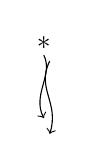
\begin{tikzpicture}[x=0.25cm,y=0.25cm]
\node at (0,4.6) {$*$};
\draw[->] (0,4) .. controls (0.5,3) and (-0.6,2) .. (0,0.8);
\draw[->] (0.3,3.7) .. controls (-0.4,2.3) and (0.8,1.6) .. (0.3,0);
\end{tikzpicture}}}
\diagram{\begin{tikzcd}[ampersand replacement=\&]
Y \& Y' \arrow[l,"g"'] \arrow[d,"i'"]\\
X \arrow[u,"\unsure{i}"] \& X' \arrow[l,"f"]
\end{tikzcd}}
\[
g^*(\mathbb{R}i^!)\longrightarrow(\mathbb{R}i'^!)f^*
\]
un isom. Tensorisant par
$T_{Y'/Y}$ et \unsure{shiftant} les degrés, il
revient au même de prouver que l'hom
naturel
\[
(\mathbb{R}^!g\deleted{\unsure{*}})(\mathbb{R}i^!)\longrightarrow(\mathbb{R}i'^!)(\mathbb{R}^!f)
\]
est un isom. Or \deleted{\unsure{par}} les th. de dualité
pour $f,g,i,i'$ nous disent essentiellement que
les deux mbs sont ``adjoints'' de
$(\mathbb{R}_!i)(\mathbb{R}_!g)$ et de $(\mathbb{R}_!f)(\mathbb{R}_!i')$, or ces derniers
sont canoniquement isomorphes. Il faut évidemment
prouver que l'\deleted{hom} isom \deleted{\unsure{ainsi}} précédent est bien
``adjoint'' de l'hom $(*)$, ce que je \unsure{suppose} fait.
Je vois un \unsure{ennui} de \unsure{degré|degrés}, car il faudrait
savoir, lorsqu'on prend un \unsure{complexe} $F\in\operatorname{Ob}\mathrm{C}(X)$,
\mspage{57}

\scanpage{59}
\mspage{- 26 -}

In $\underline{S}$, roots exist, and hence this natural transformation
induces a unique map:
\[
\varphi_{G,D}:\mathrm{Rr}\operatorname{Hom}_{\underline{A}}(G,D(-))
\longrightarrow\operatorname{Hom}_{\underline{A}}(G,\mathrm{Rr}\,D).
\]
We are interested in the case where $\underline{D}$ is a directed system.
(See \S 4, Ex. iii).) Let $D(i)=A_i$, $i\in\underline{D}$. Then
\[
\varphi_{G,D}:\operatorname{dir\,lim}\operatorname{Hom}_{\underline{A}}(G.A_i)
\longrightarrow\operatorname{Hom}_{\underline{A}}(G,\operatorname{dir.\,lim}A_i).
\]

\uline{5.2.} \uline{Definition:} $G\in\underline{A}$ is called \uline{small} if for every directed
system $D:\underline{D}\longrightarrow\underline{A}$, the above morphism $\varphi_{G,D}$ is a monomorphism.
If there is a generating family (\S 1,vii) of small objects, then
we say that $\underline{A}$ \uline{has enough} small objects. \uline{Cosmall} objects are
defined dually.

\uline{5.3.} \uline{Examples:} In the category of sets or topological spaces,
the set consisting of a single point is a small generator. In
the category of abelian groups, $Z$ is a small generator. In
the category of torsion abelian groups, $\{Z_p\}$ is a generating
family of small objects. In the category of modules over $R$,
$R$ is a small generator. Dual statements hold in the dual
categories. For a characterization of small objects in special
categories, see 6.4. below.
\mspage{58}

\scanpage{60}

que \inserted{4 \deleted{\unsure{foncteurs}}\unsure{foncteurs} qui interviennent \unsure{au} \unsure{départ}}
les deux mbs de ces \deleted{appliqués} à $F$, sont
bien tous bornés \inserted{en \unsure{haut}}, ce qui ne semble
nullement clair. Mais par passage à la limite,
\inserted{par le th. de changement de base \unsure{connu}}
on peut supposer $X$ est de type fini sur $Z$.
\deleted{et \unsure{lisse} \unsure{sur} \unsure{affine} de la forme $\operatorname{Spec}Z[t_1,\unsure{\ldots|--},t_n]$.}

Alors le th de la dimension cohomologique
nous apprend que les
\deleted{$\unsure{\mathbb{R}}\,\unsure{cohomol}\,\unsure{\Gamma'}$}
\inserted{$(\mathbb{R}j_*)$}, $j$ ouvert
\unsure{Affinement} ! \deleted{\unsure{$\mathbb{R}$}}, \deleted{\unsure{ne} \unsure{dépend} \unsure{pas} \unsure{de} $\unsure{X^c}$ \unsure{peut-être}
\unsure{des} \unsure{raisons} pour \unsure{des} \unsure{coefficients} de $\unsure{2|l}$-torsion !!!}

! Ref exposé d'Artin.
\mspage{59}

\scanpage{61}
\mspage{- 24 -}

\uline{4.17} \uline{Proposition:} $\underline{F}_\ell(\underline{A},\underline{B})$ (resp., $\underline{F}_r(\underline{A},\underline{B})$) is left (resp.,
right) closed in $\underline{F}(\underline{A},\underline{B})$.

\uline{Proof:} We treat the case of left roots. Suppose
$D:\underline{D}\longrightarrow\underline{F}_\ell(\underline{A},\underline{B})$ is such that $\mathrm{Lr}_{\underline{D}}D$ exists in $\underline{F}(\underline{A},\underline{B})$. It
is sufficient to show that $\mathrm{Lr}_{\underline{D}}D\in\underline{F}_\ell(\underline{A},\underline{B})$, i.e., $\mathrm{Lr}_{\underline{D}}D$
preserves left roots of type $\underline{D}_\alpha$ for all $\alpha$. So, let
$D_\alpha:\underline{D}_\alpha\longrightarrow\underline{A}$ be such that $\mathrm{Lr}\,D_\alpha\in\underline{A}$ exists. Write
$D(i)=F_i\in\underline{F}(\underline{A},\underline{B})$ for $i\in\underline{D}$ and $D_\alpha(j)=A_j\in\underline{A}$ for $j\in\underline{D}_\alpha$.
Then we must show that $[\mathrm{Lr}_{\underline{D}}F_i](\mathrm{Lr}_{\underline{D}_\alpha}A_j)=\mathrm{Lr}_{\underline{D}_\alpha}[(\mathrm{Lr}_{\underline{D}}F_i)(A_j)]$.
Consider $D*D_\alpha:\underline{D}\times\underline{D}_\alpha\longrightarrow\underline{B}$, where $D*D_\alpha(i,j)=F_i(A_j)$.
Then, by 4.3
\[
\begin{aligned}
\mathrm{Lr}_{\underline{D}\times\underline{D}_\alpha}F_i(A_j)
&=\mathrm{Lr}_{\underline{D}}[\mathrm{Lr}_{\underline{D}_\alpha}(F_i(A_j))]\\
&=\mathrm{Lr}_{\underline{D}}[F_i(\mathrm{Lr}_{\underline{D}_\alpha}(A_j)]
\quad\text{since }F_i\in\underline{F}_\ell(\underline{A},\underline{B})\\
&=[\mathrm{Lr}_{\underline{D}}F_i](\mathrm{Lr}_{\underline{D}_\alpha}(A_j))
\end{aligned}
\]
since roots in $\underline{F}(\underline{A},\underline{B})$ are computed objectwise.

On the other hand,
\[
\begin{aligned}
\mathrm{Lr}_{\underline{D}\times\underline{D}_\alpha}F_i(A_j)
&=\mathrm{Lr}_{\underline{D}_\alpha}[\mathrm{Lr}_{\underline{D}}(F_i(A_j))]\\
&=\mathrm{Lr}_{\underline{D}_\alpha}[(\mathrm{Lr}_{\underline{D}}F_i)(A_j)].
\end{aligned}
\]
Hence, $\mathrm{Lr}_{\underline{D}}F_i$ preserves roots of type $\underline{D}_\alpha$ for all $\alpha$.
\mspage{60}

\scanpage{62}
\mspage{\uline{23}}
\uline{Th. de dualité globale pour un morphisme lissement compactifiable.}

Le morphisme $f:X\mathbin{\unsure{-|\longrightarrow}}Y$ sera dit \uline{lissement compactifiable} si on peut trouver une $Y$-immersion $i:X\mathbin{\unsure{-|\longrightarrow}}X'$, où $X'$ est lisse et compactifiable sur $Y$ (par ex. propre sur $Y$!). Par exemple, si $f$ est quasi-projectif et si $Y$ admet un faisceau inversible ample, \unsure{nous} \unsure{on sait|savons} que $X$ se plonge dans un $\mathbf P^n_Y$, donc il est lissement compactifiable.

Supposons $X$ lissement compactifiable, et choisissons une immersion $i:X\mathbin{\unsure{\lhook\joinrel-|\hookrightarrow}}X'$ comme dans la définition.

\diagram{\begin{tikzcd}[ampersand replacement=\&]
X \arrow[r,hook,no head,"i"] \arrow[d,no head,"f"'] \& X' \arrow[dl,no head,"f'"]\\
Y \&
\end{tikzcd}}

Définissons un foncteur
\[
\deleted{\unsure{\mathbb{R}f^!}}
\qquad \mathbb{R}f^!:\mathrm D^+(Y)\mathbin{\unsure{-|\longrightarrow}}\mathrm D^+(X)
\]
par
\[
(*)\qquad \mathbb{R}f^!\deleted{\unsure{(F)}}=(\mathbb{R}\unsure{i|f}^!)(\mathbb{R}f'^!)
\]
où $\mathbb{R}f'^!$ est défini \unsure{---}, et $\mathbb{R}i^!$ \unsure{dans} \unsure{---}.
Conjuguant les th. de dualité pour $f'$ et pour $i$, on trouve un
\mspage{61}

\scanpage{63}
\mspage{33}
subcategory determined by functors $F$ which, for every open set $U$ and every strong covering $\underline U=\{U_i\}$ of $U$, satisfy
\[
F(U)=\mathrm{Lr}\,F\circ D_{\underline U}\;(=\operatorname{inv\,lim}F(U_i))
\]
is called the category of \uline{sheaves on} $X$ \uline{with values in} $\underline A$. It will be denoted by $\underline S(X,\underline A)$.

\uline{Remarks}: The following are equivalent definitions of a sheaf:

i) $F$ preserves inverse limits of inclusions of finitely right complete subcategories of $\underline T$.

ii) Let $\underline U=\{U_i\}$ be an arbitrary covering of an open set $U$. Then $F(U)$ is the left root of the diagrams.
\diagram{\begin{tikzcd}[ampersand replacement=\&]
F(U_i) \arrow[r] \& F(U_i\cap U_j) \& F(U_i) \arrow[l]
\end{tikzcd}}
(cf. Grothendieck [7].)

iii) If $\underline A$ has direct products,then $F(U)$ is the difference kernel of the two obvious morphisms of $\prod F(U_i)$ into $\prod F(U_i\cap U_j)$.

iv) For every $X\in\underline A$, $\operatorname{Hom}_{\underline A}(X,F(-))$ is a sheaf of sets in the usual meaning of sheaf. (See Godement [5].)

We wish to prove that $\underline S(X,\underline A)$ is a right reflective subcategory of $\underline P(X,\underline A)$. In order to do so we must begin with some preliminary constructions and lemmas.
\mspage{62}

\scanpage{64}
isom. bifonctoriel
\[
\boxed{\operatorname{Hom}(F^\bullet,\mathbb{R}f^!(G^\bullet))
\xrightarrow{\sim}
\operatorname{Hom}(\mathbb{R}f_{\unsure{!|*}}F^\bullet,G^\bullet)}
\]
\[
(F^\bullet\in\operatorname{Ob}\mathrm D^b(X),\quad G^\bullet\in\operatorname{Ob}\mathrm D^+(Y)).
\]

\uline{Lorsque} $X$ \uline{est lisse sur} $Y$, on a un isom. canonique entre $\mathbb{R}f^!$ défini par $(*)$, et $\mathbb{R}f^!$ défini directement en termes de $f$ lisse, \unsure{donné} par $\unsure{\sigma}$ : \unsure{une factorisation}.
\margin{\unsure{à prouver|à préciser}}
\margin{\figure{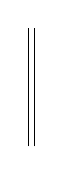
\begin{tikzpicture}\draw (0,0)--(0,1.5);\draw (.08,0)--(.08,1.5);\end{tikzpicture}}}
C'est essentiellement le \uline{th. de \deleted{dualité locale}\inserted{pureté \unsure{absolue}}} pour $f:X\longrightarrow Y$.
[N.B. C'est pour avoir ce résultat que l'on a dû définir $f^!(X)$ avec le \unsure{droit|décal.} de translation sur les degrés\unsure{\ldots}].
Ceci dit, le \deleted{\uline{\unsure{isom}}}\inserted{\uline{hom}} de dualité défini ici par la composition $f=f'i$ n'est autre que celui défini directement \deleted{\unsure{au}} \unsure{moyen} de $f$ : c'est essentiellement le ``th. de compatibilité entre classes fondamentales locales et globales'' auquel il a été fait allusion déjà.
\mspage{63}

\scanpage{65}
\mspage{32}
Chapter II. \uline{Sheaves}

\S\ 1. \uline{Existence Theorems}: Let $X$ be a set. The collection of all subsets of $X$ can be considered as the collection of objects of a category $\underline X$ where there is a unique morphism $A\longrightarrow B$ if and only if $B\supset A$. (Note the reversal of order.) If $T_X$ is a topology on $X$ (i.e., a collection of open sets) then $T_X$ determines a full subcategory $\underline T_X$ (or just $\underline T$ when only one space is being considered) of $\underline X$. $\underline X$ and $\underline T$ are clearly small categories. $\underline X$ is complete, for a left (resp., right) root in $\underline X$ is simply a union (resp., intersection), while $\underline T$ is left complete and finitely right complete.

Let $\underline U=\{U_i\}$ be a collection of open sets with $U=\bigcup U_i$. If $\underline U$ is closed under finite intersections (i.e., the subcategory of $\underline T$ determined by $\underline U$ is finitely right complete), then $\underline U$ is called a \uline{strong covering} of $U$. Note that if $D_{\underline U}:\underline U\longrightarrow\underline T$ is the inclusion functor then $U=\mathrm{Lr}\,D_{\underline U}$.

1.1 \uline{Definition}: For any category $\underline A$, the functor category $\underline F(\underline T_X,\underline A)$ will be called the category of \uline{presheaves on} $X$ \uline{with values in} $\underline A$. It will be denoted by $\underline P(X,\underline A)$. The full
\mspage{64}

\scanpage{66}
Pour se sentir à l'aise du point de vue \deleted{\unsure{des variances}} variances, on doit se rendre compte que la définition de $\mathbb{R}f^!$ et de l'hom de dualité ne dépend pas, essentiellement, de la factorisation choisie.
\inserted{L'argument qui suit est dû à Lichtenbaum (dans le cas de la dualité des faisceaux cohérents).}
Si on en a deux par $X'$, $X''$, on en a une autre avec $X'''=X'\times_Y X''$, et pour définir un isom. can. entre $\mathbb{R}^!_{i'}f^{\deleted{\unsure{!}}}_{\deleted{\unsure{*}}}$ et $\mathbb{R}^!_{i''}f^{\deleted{\unsure{!}}}_{\deleted{\unsure{*}}}$, compatible aux hom de dualité, on \uline{\unsure{le définira}} entre \deleted{\unsure{respect.}} \unsure{un} chacun et $\mathbb{R}^!_{i'''}f_{\unsure{*}}$, ce qui nous ramène à une situation où on a un hom \inserted{\uline{lisse}} $X''\xrightarrow{g}X'$ tel que $i'=gi''$.

\margin{\diagram{\begin{tikzcd}[ampersand replacement=\&]
\& X''' \arrow[ddl] \arrow[ddr] \&\\
\& X \arrow[u,"\deleted{\unsure{i}}"] \arrow[dl] \arrow[dr,no head] \&\\
X' \& \& X''
\end{tikzcd}}}

\diagram{\begin{tikzcd}[ampersand replacement=\&]
\& X'' \arrow[r,"g"] \arrow[dr,no head,"f''"'] \& X' \arrow[d,no head,"f'"]\\
X \arrow[ur,"i''"] \arrow[urr,no head,"i'" description] \arrow[rr,"f"'] \& \& Y
\end{tikzcd}}

Utilisant $\mathbb{R}^!f''\mathbin{\unsure{\cdot}}\mathbb{R}^!(f')\simeq(\mathbb{R}^!g)(\mathbb{R}^!f')$, on est ramené au cas où $X'=Y$ et $f'=\operatorname{id}_Y$.
Changeant les notations, on est ramené au cas où on a $q:X\longrightarrow Y$ lisse, et $Y'\mathbin{\underset{i}{\unsure{-|\longrightarrow}}}Y$ : imm., et où on a un \deleted{\unsure{morphisme}}\inserted{$Y$-morphisme} \deleted{\unsure{de}} de $\unsure{X'}$ \unsure{sur} $X$, i.e. une section de $\sigma$ de $X'=X\times_Y Y'$ sur $Y'$.

\margin{\diagram{\begin{tikzcd}[ampersand replacement=\&]
X \arrow[d,"q"'] \& X' \arrow[l,hook',"j"'] \arrow[d,"q'"] \arrow[d,bend left=45,"\sigma"]\\
Y \& \deleted{\unsure{X'}}\inserted{Y'} \arrow[l,hook',"i"{description}, "\text{imm.}"']
\end{tikzcd}}}
\margin{$q,q'$ lisses, $i,j,\unsure{\sigma}$ immersions.}
\mspage{65}

\scanpage{67}
- \mspage{31} -
of subobjects of $B$ and any $g:G\longrightarrow\mathrm{l.u.b}\,\{A_i\}$ there is a $g':G\longrightarrow A_i$, for some $i$, such that $f_i g'=g$, then $G$ is small. If, in addition, $G$ is projective, then $\varphi_{G,D}$ is a bijection for all directed systems $D$. The dual characterization holds for cosmall objects.

\uline{Proof}: Let $k_{ji}:B_i\longrightarrow B_j$ be any directed system with $k_j:B_j\longrightarrow\operatorname{dir\,lim}B_j$ the induced morphisms. Let $h:G\longrightarrow B_i$ be such that $k_i h:G\longrightarrow\operatorname{dir\,lim}B_j$ is the zero morphism. We must show that $h\in\operatorname{Hom}_{\underline A}(G,B_i)$ represents zero in $\operatorname{dir\,lim}\operatorname{Hom}_{\underline A}(G,B_j)$. Since $k_i h=0$, $k_i h$ factors through $\operatorname{Ker}k_i=\operatorname{dir\,lim}\operatorname{Ker}k_{ji}=\mathrm{l.u.b.}(\operatorname{Ker}k_{ji})$. Since $\{\operatorname{Ker}k_{ji}\}$ is an increasing direct family of subobjects of $A_i$, $k_i h$ factors through some $\operatorname{Ker}k_{ji}$, $j\geq i$. Hence $k_{ji}h=0$ for some $j$. q.e.d.

Suppose now that $G$ is also projective. Given any morphism $h:G\longrightarrow\operatorname{dir\,lim}B_i=\mathrm{l.u.b.}\,(\operatorname{Im}k_i)$, $h$ factors through some $\operatorname{Im}k_i$. Since $B_i\longrightarrow\operatorname{Im}k_i$ is an epimorphism, $h$ lifts to $h':G\longrightarrow B_i$. The class represented by $h'$ in $\operatorname{dir\,lim}\operatorname{Hom}_{\underline A}(G,B_i)$ is mapped by $\varphi_G$ onto $h$. Hence $\varphi_G$ is a bijection.
\mspage{66}

\scanpage{68}
À \deleted{prouver que}\inserted{définir un} isom de foncteurs
\[
(\unsure{A|\alpha})\qquad \mathbb{R}i^!\simeq
\deleted{\unsure{(\mathbb{R}^!g)}}\,\mathbb{R}^{\deleted{\unsure{!}}}(j\sigma)^!\mathbb{R}^!g
\]
et une commutativité de diagrammes reliant les $\operatorname{Tr}_i$\deleted{\unsure{et}}, $\operatorname{Tr}_g$, $\operatorname{Tr}_{j\sigma}$.
Comme on a un isom
\[
\mathbb{R}(j\sigma)^!\simeq \mathbb{R}\sigma^!\,\mathbb{R}j^!
\]
provenant de
\[
(j\sigma)^!\simeq\sigma^!j^!
\]
on définira $(\unsure{A|\alpha})$ comme \deleted{déduit de}
\[
\mathbb{R}^{\deleted{\unsure{!}}}\deleted{\unsure{\sigma}}i^!
\simeq \mathbb{R}^{\deleted{\unsure{!}}}\sigma^!(\mathbb{R}j^!\,\mathbb{R}^!g)
\]
déduit des isom suivants
\[
\left\{\begin{aligned}
(\mathbb{R}^!\unsure{g'})(\mathbb{R}i^!)&\simeq(\mathbb{R}^{\deleted{\unsure{!}}}j^!)(\mathbb{R}^!g) &&(a)\\
\deleted{\unsure{\mathbb{R}^!\operatorname{id}_{\mathrm D^+(Y')}}}\quad
\mathbb{R}^!\operatorname{id}_{Y'}&\simeq(\mathbb{R}\sigma^!)(\mathbb{R}^!g') &&(b)
\end{aligned}\right.
\]
d'où
\[
\begin{aligned}
\mathbb{R}i^!&=\deleted{\unsure{(\mathbb{R}i^!)}}
(\mathbb{R}^!\operatorname{id}_{Y'})(\mathbb{R}i^!)
\underset{\inserted{\text{après : $(a)$}}}{\simeq}
\deleted{\unsure{\mathbb{R}i^!}}\mathbb{R}\sigma^!\,
\underbrace{\mathbb{R}^!g'\,\mathbb{R}i^!}_{\deleted{\unsure{(a)}}}\\
&\simeq
\inserted{\text{\figure{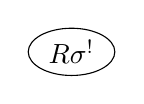
\begin{tikzpicture}[baseline=-.5ex]
\draw (0,0) ellipse (.55 and .3);
\node at (0,0) {$\mathbb{R}\sigma^!$};
\end{tikzpicture}}}}
(\mathbb{R}j^!\,\mathbb{R}^!g\,\deleted{\unsure{\mathbb{R}i^!}})
\end{aligned}
\]
ce qu'on voulait définir. Il faut donc définir $(a)$ et $(b)$. Or $(b)$ est un cas particulier du ``th. de compatibilité des classes fond locales et globales'' (lorsque l'un des \unsure{$Y$-schémas} \unsure{lisses envisagés} est isom. à la base \unsure{\ldots}).
\mspage{67}

\scanpage{69}
- \mspage{30} -
v) If $\underline A$ is right perfect and has a generator, then $\underline C$ has enough injectives (i.e., every object is a subobject of an injective object.)

\uline{Proof}: i) Since $\underline A$ is right complete, by 4.2, $\underline F(\underline B,\underline A)$ is right complete and hence, by 4.14, $\underline C$ is right complete.

ii) If $\underline A$ has a generator $G$, then by Freyd [3] $\underline F(\underline B,\underline A)$ has a generator; namely $\widetilde G=\coprod_{B\in\underline B}F_B$ where, for $B\in\underline B$, $F_B$ is the functor such that for any $B'\in\underline B$, $F_B(B')=\coprod_{\operatorname{Hom}(B,B')}G$. Hence, by 3.2, $R(\widetilde G)$ is a generator for $\underline C$.

iii) If $\underline A$ is abelian, then $\underline F(\underline B,\underline A)$ is abelian and hence, by 6.2, $\underline C$ is abelian.

iv) If $\underline A$ is right perfect, then so is $\underline F(\underline B,\underline A)$ since limits in $\underline F(\underline B,\underline A)$ are computed objectwise and a sequence of functors is exact if and only if it is e xact on each \unsure{object}. Hence, by 6.2., $\underline C$ is right perfect.

v) Grothendieck [6]. Théorème 1.10.1 shows that if $\underline C$ is right perfect and has a generator, then $\underline C$ has enough injectives. Alternatively, injective envelopes of functors exist in $\underline F(\underline B,\underline A)$ and hence by 3.3, there are \unsure{injectives} in $\underline C$. If $C\longrightarrow F$ is a monomorphism into an injective in $\underline F(\underline B,\underline A)$, then $C=R(C)\longrightarrow R(F)$ is a monomorphism into an injective in $\underline C$.

\uline{Remark}: Propositions 6.2 and 6.3 have duals by replacing right everywhere by left and vice versa.

Finally, we give a characterization of small objects in a right perfect category. (\S5.2).

\uline{6.4.}\quad\uline{Proposition}: Let $\underline A$ be a right perfect category, and let $G\in\underline A$. If for any increasing directed family $\{f_i:A_i\longrightarrow B\}$
\mspage{68}

\scanpage{70}
d'autre part $(a)$ s'écrit, modulo \uline{shift} de degré et tensorisation par \deleted{\unsure{la $\Omega^d$}} un $\underline\Omega^d_{X'/Y'}$
(NB $\underline\Omega^d_{X'/Y'}\simeq\underline\Omega^d_{X/Y}\otimes_{\mathcal O_X}\mathcal O_{X'}$)
\[
g'^*(\mathbb{R}i^!)\simeq(\mathbb{R}j^!)g^*
\]
et résulte donc simplement du \uline{th. de changement de base lisse}.

Cela définit l'isom de foncteurs qu'on voulait définir. Il reste à vérifier la compatibilité avec les hom de dualité, ce qui n'offre pas de difficultés, et est laissé au lecteur \unsure{\ldots}

\uline{Remarques}\quad a) Pour se sentir à l'aise, il aurait fallu vérifier que les isom ainsi définis entre les foncteurs $\mathbb{R}^!f$, par des immersions différentes dans des $X'$ lisses $/Y$, satisfont la condition naturelle de transitivité.
Nous \unsure{l'admettrons|l'admettons} --- la vérification ne \unsure{saurait} être particulièrement triviale. Cette compatibilité et de nombreuses autres seront \unsure{énoncées} plus loin dans le ``\uline{formulaire}''.
\mspage{69}

\scanpage{71}
- \mspage{29} -
Since $\operatorname{Coim}f=\operatorname{Im}f$, it follows that $\operatorname{Coim}'f=\operatorname{Im}'f$.

ii) Let $0\longrightarrow D'\longrightarrow D\longrightarrow D''\longrightarrow0$ be an exact sequence of directed systems in $\underline A'$ with $D'(i)'=A_i'$, etc.
(i.e., for for each $i\in\underline D$, $0\longrightarrow A_i'\longrightarrow A_i\longrightarrow A_i''\longrightarrow$ is exact in $\underline A'$.

Then, by 4.7,
\[
*)\quad\operatorname{dir\,lim}A_i'\longrightarrow\operatorname{dir\,lim}A_i
\longrightarrow\operatorname{dir\,lim}A_i''\longrightarrow0
\]
is exact in $\underline A'$. We must show it is also exact on the left. Now, since $I_{\underline A\underline A'}$ has a left adjoint,
\[
0\longrightarrow I_{\underline A\underline A'}(A_i')
\longrightarrow I_{\underline A\underline A'}(A_i)
\longrightarrow I_{\underline A\underline A'}(A_i'')
\]
is exact in $\underline A$. (In general it is not exact on the right in $\underline A$).
Hence, since $\underline A$ is right perfect,
\[
0\longrightarrow\operatorname{dir\,lim}I_{\underline A\underline A'}(A_i')
\longrightarrow\operatorname{dir\,lim}I_{\underline A\underline A'}(A_i)
\longrightarrow\operatorname{dir\,lim}I_{\underline A\underline A'}(A_i'')
\]
is exact. Since $R$ is an exact functor, the sequence remains exact after applying $R$. But, by 4.14,
\[
R[\operatorname{dir\,lim}I_{\underline A\underline A'}(A_i')]
=\operatorname{dir\,lim}A_i'
\]
etc. Hence, the sequence *) is exact on the left.

\uline{6.3.}\ \uline{Theorem}: Let $\underline C$ be a full subcategory of a functor category $\underline F(\underline B,\underline A)$ where $\underline A$ is right complete. Suppose $R:\underline F(\underline B,\underline A)\longrightarrow\underline C$ is a right reflection. Then

i) $\underline C$ is right complete

ii) If $\underline A$ has a generator, then so does $\underline C$.

Suppose further that $\underline A$ is abelian, $\underline C$ is left closed, and $R$ is exact. Then

iii) $\underline C$ is abelian.

iv) If $\underline A$ is right perfect, then so is $\underline C$.
\mspage{70}

\scanpage{72}
b) Dans la définition du foncteur $\mathbb{R}^!f$, on n'a pas utilisé le fait que $f$ soit compactifiable, mais uniquement qu'il soit ``lissifiable''; \deleted{\unsure{par une immersion}} dans un $X'$ lisse de dim relative sur $Y$ finie.
\inserted{L'hyp ``$f$ est compactifiable'' ne sert que pour pouvoir écrire $\mathbb{R}_!f(\mathbb{R}^!f)$ et l'hom de dualité correspondant.}
\deleted{\unsure{À généraliser}}
Cela semble \unsure{un|aussi} \unsure{pt technique} important de trouver une définition directe de $\mathbb{R}^!f$ pour $f$ loc de type fini de dim relative bornée, tout comme le pb de définir $\mathbb{R}_!f$ sans supposer $f$ compactifiable, mais seulement loc. de type fini (ce qui semble l'hyp naturelle).
Il y a lieu, \deleted{\unsure{si $f$ est défini}}\inserted{chaque fois que} $\mathbb{R}_!f$ et $\mathbb{R}^!f$ sont définis, de trouver un \uline{hom}
\[
\uline{\text{trace}}\quad
\operatorname{Tr}_f:(\mathbb{R}_!f)(\mathbb{R}^!f)\mathbin{\unsure{-|\longrightarrow}}
\operatorname{id}_{\mathrm D^+(Y)}
\]
qui devrait donner lieu, du moins si $f$ est de \uline{type fini}, à un ``\uline{hom de dualité}'' qui est un \uline{isom}!
\mspage{71}

\scanpage{73}
- \mspage{28} -
Since direct limits are exact, taking the direct limit over $j$ yields $0\longrightarrow\operatorname{dir\,lim}(\operatorname{Ker}f_{ji})\longrightarrow A_i\longrightarrow A_o$.
Hence $\operatorname{Ker}f_i=\operatorname{dir\,lim}(\operatorname{Ker}f_{ji})$.

c) In general, if $g=\operatorname{dir\,lim}A_i\longrightarrow Y$, let $v_i=gf_i:A_i\longrightarrow Y$. Then $\operatorname{Ker}g:\mathrm{l.u.b.}\ \operatorname{Im}(f_i\circ\operatorname{ker}v_i)$.
Similarly, if $h:X\longrightarrow A_i$ is given, then $\operatorname{Ker}(f_i h)=\mathrm{l.u.b.}\operatorname{Ker}(f_{ji}\circ h)$. Thus Amitsur's conditions L2.2 and L2.3 of [1] \unsure{.:} are consequences of right perfection.

\uline{6.2.}\ \uline{Proposition}: Let $\underline A'$ be a full, left closed subcategory of an abelian category $\underline A$. If $\underline A'$ is right reflective and the reflection $R:\underline A\longrightarrow\underline A'$ is exact (i.e. preserves kernels and cokernels), then

i) $\underline A'$ is abelian

ii) If $\underline A$ is right perfect, then $\underline A'$ is right perfect.

\uline{Proof}: i) The proof of this part was pointed out by F. William Lawvere. Since $\underline A'$ is full, $\underline A'$ is additive. Since $\underline A'$ is left closed and $\underline A$ has kernels and finite direct products, $\underline A'$ has kernels and finite direct products. Since $\underline A'$ is right reflective and full and $\underline A$ has cokernels, by 4.14, $\underline A'$ has cokernels. If $f$ is a morphism in $\underline A'$, let $\operatorname{Ker}'f$ (resp., $\operatorname{Ker}f$) denote the kernel of $f$ in $\underline A'$ (resp., $\underline A$). Similarly, for $\operatorname{Cok}'f$, etc.
To verify Grothendieck's axioms [6] for an abelian category, it remains to show that $\operatorname{Coim}'f=\operatorname{Im}'f$. Since $\underline A'$ is left closed, $\operatorname{Ker}'f=\operatorname{Ker}f$, and by 4.14, $\operatorname{Cok}'f=R(\operatorname{Cok}f)$. Hence
\[
\operatorname{Coim}'f=\operatorname{Cok}'(\operatorname{ker}'f)
=R[\operatorname{Cok}(\operatorname{ker}f)]=R(\operatorname{Coim}f)
\]
and, since $R$ is exact,
\[
\operatorname{Im}'f=\operatorname{Ker}'(\operatorname{cok}'f)
=\operatorname{Ker}'[R(\operatorname{cok}f)]
=R[\operatorname{Ker}(\operatorname{cok}f)]=R(\operatorname{Im}f).
\]
\mspage{72}

\scanpage{74}
\mspage{\uline{23} bis}
\uline{L'hom de dualité pour un sous-préschéma \deleted{\unsure{lisse}} d'un préschéma lisse}

\inserted{Définir $\mathbb{R}i^!$ pour une \uline{immersion} \deleted{\unsure{ferm.}}}
L'hom $(\mathbb{R}i_!)\mathbb{R}i^!(F^\bullet)\longrightarrow F^\bullet$

\diagram{\begin{tikzcd}[ampersand replacement=\&]
Y \arrow[r,hook,no head,"i"',"{(d)}" description] \arrow[dr,"g"',"{(r-d)}" description] \& X \arrow[d,"f","{(r)}"']\\
\& S
\end{tikzcd}}

\[
\mathbb{R}i_!\bigl(\underbrace{\mathbb{R}i^!(T_{X/S})}_{\underset{\downarrow}{\phantom{\mathbb{R}i^!}}\ \text{\uline{\unsure{redéfinir}}}}\bigr)
\simeq\deleted{\unsure{\mathbb{R}_!g_*}}
\inserted{\mathbb{R}i_!(T_{Y/S}[-2d])}
\longrightarrow \mathbb{R}_!f_*(T_{X/S})
\]
\[
\mathbb{R}_!\unsure{i|g}_*(T_{Y/S}[-2d])\longrightarrow \mathbb{R}_!f_*(T_{X/S})
\]
\[
\mathbb{R}_!g_*(T_{Y/S})[-2d]\longrightarrow \mathbb{R}_!f_*(T_{X/S})
\]
\[
\deleted{\unsure{\mathbb{R}^{2r}}}\qquad
\mathbb{R}_!^{i\unsure{+|-}2d}g_*(T_{Y/S})\longrightarrow
\mathbb{R}_!^{i\deleted{\unsure{+2d}}}f_*(T_{X/S})
\]
Faisons $i=2r\deleted{\unsure{-2d}}$, on trouve \unsure{)}
\[
\mathbb{R}_!^{2(r-d)}g_*(T_{Y/S})\longrightarrow T_{X/S}
\]

a) Cet hom est compatible avec les hom trace.

b) Plus généralement, on a pour tt $G$ sur $S$ un isom de foncteurs
\[
\deleted{\mathbb{R}^!g^{\unsure{*}}(G)\simeq \mathbb{R}i^!\mathbb{R}f^!(G)}
\]
\[
\mathbb{R}g^!(G)\simeq \mathbb{R}i^!\mathbb{R}f^!(G)
\]
\mspage{73}

\scanpage{75}
- \mspage{210} -
\margin{n$^\circ$ 391}
\[
\begin{aligned}
\alpha_1&=\tfrac12(\varepsilon_1+\varepsilon_8)-\tfrac12(\varepsilon_2+\varepsilon_3+\varepsilon_4+\varepsilon_5+\varepsilon_6+\varepsilon_7),\quad
\alpha_2=\varepsilon_1+\varepsilon_2,\\
\alpha_3&=\varepsilon_2-\varepsilon_1,\quad
\alpha_4=\varepsilon_3-\varepsilon_2,\quad
\alpha_5=\varepsilon_4-\varepsilon_3,\quad
\alpha_6=\varepsilon_5-\varepsilon_4,\quad
\alpha_7=\varepsilon_6-\varepsilon_5,\\
\alpha_8&=\varepsilon_7-\varepsilon_6.
\end{aligned}
\]
Il est clair, en vertu de (I), que ce sont des racines de $R$, et qu'elles sont $>0$ pour l'ordre considéré. D'autre part, pour cet ordre, les racines positives sont les $\varepsilon_j\pm\varepsilon_i$ pour $i<j$ et les racines $\tfrac12(\varepsilon_8+\sum_{i=1}^7(-1)^{\unsure{\vartheta|\delta}(i)}\varepsilon_i)$ avec $\sum_{i=1}^7\unsure{\vartheta|\delta}(i)$ pair. Montrons que ces racines sont combinaisons linéaires des $\alpha_i$ à coefficients tous $>0$. Pour les racines $\varepsilon_j\pm\varepsilon_i$ avec $1\leq i<j\leq7$, cela résulte du calcul fait pour le système de type $D_7$, (n$^\circ$ 8). Il en est de même de $\varepsilon_1+\varepsilon_8$ par l'expression de $\alpha_1$, puis, par récurrence sur $i$, de $\varepsilon_8+\varepsilon_i=(\varepsilon_8+\varepsilon_{i-1})+(\varepsilon_i-\varepsilon_{i-1})$ pour $2\leq i\leq7$. En considérant ensuite l'expression $2\alpha_1+\alpha_3$, on obtient $\varepsilon_8-\varepsilon_7$ comme combinaison des $\alpha_i$ à coefficients $\geq0$, puis par récurrence descendante sur $i$, $\varepsilon_8-\varepsilon_i=(\varepsilon_8-\varepsilon_{i+1})+(\varepsilon_{i+1}-\varepsilon_i)$ pour $1\leq i\leq6$. En ajoutant à $\alpha_1$ des éléments $\varepsilon_i+\varepsilon_j$ avec $2\leq i<j\leq7$, on obtient toutes les racines de la forme $\tfrac12(\varepsilon_1+\varepsilon_8)+\tfrac12(\sum_{i=2}^7(-1)^{\unsure{\vartheta|\delta}(i)}\varepsilon_i)$ avec $\sum_{i=2}^7\unsure{\vartheta|\delta}(i)$ pair ; enfin, $\alpha_1+\alpha_2$ a la même forme que $\alpha_1$ sauf qu'on y a permuté $\varepsilon_1$ et $\varepsilon_2$, et en lui ajoutant des éléments $\varepsilon_i+\varepsilon_j$ avec $1\leq i<j\leq7$, $i$, $j$ distincts de $2$, on achève de prouver notre assertion. Les $\alpha_i$, $(1\leq i\leq8)$, forment donc un système de \uline{racines simples} $S$ pour $R$, (\S\ 6, n$^\circ$ 7, cor. 2 de la prop. 14). En outre, on a $(\alpha_i|\alpha_i)=2$ pour tout $i$, $(\alpha_i|\alpha_{i+1})=(\alpha_2|\alpha_4)=(\alpha_1|\alpha_3)=-1$, $(3\leq i\leq8)$, et $(\alpha_i|\alpha_j)=0$ pour tous les autres couples d'indices ; le schéma de Dynkin de $R$ est donc de type $E_8$, et $R$ est irréductible.
\mspage{74}

\scanpage{76}
qui \uline{généralise le th. de pureté relatif}
[et se déduit d'ailleurs du th de dualité globale --- cela devrait être explicité dans SGA \deleted{\unsure{4|5}}].
\margin{\figure{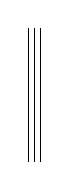
\begin{tikzpicture}\draw (0,0)--(0,1.7);\draw (.08,0)--(.08,1.7);\draw (.16,0)--(.16,1.7);\end{tikzpicture}}}
Se réduit aux formules
\[
\underline H^i_Y(f^*(G))=
\begin{cases}
0 & i\ne2d\\
g^*(G)\otimes T_{Y/X}^{-1} & \text{si }i=2d
\end{cases}
\]

Cet isomorphisme se généralise donc au cas d'un $G^\bullet$ :
\[
\mathbb{R}g^!(G^\bullet)\simeq \mathbb{R}i^!(\mathbb{R}f^!(G^\bullet))
\]
On en déduit un hom canonique
\[
\deleted{\unsure{\mathbb{R}_!f}(\mathbb{R}g^!(G^\bullet))\longrightarrow \mathbb{R}^!f}
\]
\[
\mathbb{R}_!i_*(\mathbb{R}g^!(G^\bullet))\mathbin{\unsure{-|\longrightarrow}}\mathbb{R}f^!(G^\bullet)
\]
d'où en appliquant $\mathbb{R}_!f_*$, et utilisant la transitivité
\diagram{\begin{tikzcd}[ampersand replacement=\&,column sep=large]
\mathbb{R}_!g_*(\mathbb{R}g^!(G^\bullet)) \arrow[rr] \arrow[dr,no head,"\operatorname{Tr}_g(G^\bullet)"'] \&\&
\mathbb{R}_!f_*\mathbb{R}f^!(G^\bullet) \arrow[dl,"\operatorname{Tr}_f(G^\bullet)"]\\
\& G^\bullet \&
\end{tikzcd}}
\margin{\unsure{rend} commutatif}
\mspage{75}

\scanpage{77}
- \mspage{209} -
\margin{n$^\circ$ 391}
(VII) On a déterminé ci-dessus les racines positives ; leur somme est donc :
\[
2\rho=5\varepsilon_1+3\varepsilon_2+\varepsilon_3+9\varepsilon_4
=16\alpha_1+30\alpha_2+42\alpha_3+22\alpha_4.
\]

(VIII) On vient de voir que l'on a $\Gamma(R)=\Gamma_o(R)$, l'indice de connexion est donc $1$.

(IX) La famille des exposants a $4$ termes, et puisque $h=12$, les entiers $1$, $5$, $7$ et $11$ étrangers à $12$, doivent figurer dans cette famille, (\S\ 8, n$^\circ$ 5, prop. 5); ce sont par suite tous les exposants de $W(R)$.

(X) On déduit de (IX) et du \S\ 8, n$^\circ$ 3, cor. 1 de la prop. 3 que l'ordre du groupe de Weyl $W(R)$ est :
\[
2.6.8.12=2^7.3^2=1152.
\]

(XI) Le même raisonnement qu'au n$^\circ$ 6 montre que le seul automorphisme du schéma de Dynkin $F_4$ est l'identité.

10. \uline{Système de type} $E_8$.

(I) Considérons dans $V=R^8$ le réseau $L_3$, (n$^\circ$ 4) ; l'ensemble $R$ des vecteurs $u$ de $L_3$ tels que $(u|u)=2$ est formé des vecteurs :
\[
\pm\varepsilon_i\pm\varepsilon_j,\ (i\ne j),\quad
\tfrac12\sum_{i=1}^{8}(-1)^{\unsure{\vartheta|\delta}(i)}\varepsilon_i
\]
où, (en vertu de la définition de $L_3$), la somme des $\unsure{\vartheta|\delta}(i)$ doit être \uline{paire} ; cela résulte de nouveau du fait qu'un vecteur de $R$ ne peut avoir de composante de valeur absolue $3/2$. On a vu, (n$^\circ$ 4), que $(u|v)\in Z$ quels que soient $u$, $v$ dans $R$, et le même raisonnement qu'au n$^\circ$ 5 montre que $R$ est un \uline{système de racines réduit}, ayant $n=\binom82.4+2^7=240$ éléments.

(II) Munissons $R^8$ de l'ordre \uline{opposé} à l'\uline{ordre lexicographique} défini par les $\varepsilon_i$, de sorte que pour cet ordre on a $\varepsilon_i<\varepsilon_{i+1}$ pour $1\leq i\leq7$. Considérons les $8$ vecteurs :
\mspage{76}

\scanpage{78}
On en conclut que si $F^\bullet$ \unsure{un}
\deleted{\unsure{fais}}\inserted{\unsure{cplxe}} sur
$Y$, alors \unsure{on a commutativité dans}
\diagram{\begin{tikzcd}[ampersand replacement=\&,column sep=large,row sep=large]
\uline{\operatorname{Ext}}^i(Y,F^\bullet,
 \overbrace{\mathbb{R}g^!(G^\bullet)}^{\substack{\inserted{\mathbb{R}i^!\mathbb{R}f^!(G^\bullet)}\\\Vert}})
 \arrow[r,"\Theta_g"] \arrow[d,"\Theta_i"',"\sim"]
\&
\operatorname{Ext}^i(S,\mathbb{R}_!g_*(F^\bullet),G^\bullet)
 \arrow[d,"\text{transitivité}","\sim"']
\\
\operatorname{Ext}^i(X,\mathbb{R}i_*(F^\bullet),
 \underbrace{\mathbb{R}f^!(G^\bullet)}_{\deleted{\substack{\Vert\\\unsure{\mathbb{R}i^!\mathbb{R}}}}})
 \arrow[r,"\Theta_f"]
\&
\operatorname{Ext}^i(S,\mathbb{R}_!f_*(\mathbb{R}\unsure{i_!|i_*}(F^\bullet)),G^\bullet)
\end{tikzcd}}
i.e. compte tenu de l'isom de dualité
pour $\Theta_i$ (cas. trivial) et de l'isom
de transitivité pour $f,i$ (cas. trivial aussi)
l'isom de dualité $\Theta_g$ est ``induit''
par $\Theta_f$. Kif-Kif en localisant
sur la base ----
\mspage{77}

\scanpage{79}
- \mspage{208} -
\margin{n$^\circ$ 391}
(III)\quad En vertu du \S~8, n$^\circ$ 3, formule (4), on a $h=n/\ell=12$.

(IV)\quad L'ordre de la plus grande racine est $h-1=11$, (\S~8, n$^\circ$ 5, prop. 6).
Or $\varepsilon_1+\varepsilon_4=2\alpha_1+3\alpha_2+4\alpha_3+2\alpha_4$ est d'ordre 11, et c'est donc la plus grande
racine $\widetilde{\alpha}$; elle est orthogonale à toutes les racines simples sauf $\alpha_1$ et on a
$(\widetilde{\alpha}|\alpha_1)=1$.

(V)\quad Les \uline{coracines} sont les vecteurs $\pm2\varepsilon_i^*$, $\pm\varepsilon_i^*\pm\varepsilon_j^*$ $(i\ne j)$, et
$\pm\varepsilon_1^*\pm\varepsilon_2^*\pm\varepsilon_3^*\pm\varepsilon_4^*$. Les angles des coracines étant égaux à ceux des racines
correspondantes, le système de racines $R^*$ ne peut avoir comme schéma de Dynkin
que $F_4$, (puisque le schéma de Coxeter détermine alors le schéma de Dynkin), et $R^*$
est donc isomorphe à $R$, ce que l'on peut vérifier directement en calculant les
images canoniques $\alpha_i^*$ des $\alpha_i$ qui forment un système de racines simples de $R^*$. Les
racines non orthogonales à $u=\varepsilon_1$ sont $\pm u$, $\pm\varepsilon_1\pm\varepsilon_j$, $(j\geq2)$ et
$\frac12(\pm\varepsilon_1\pm\varepsilon_2\pm\varepsilon_3\pm\varepsilon_4)$, donc sont au nombre de 30, et on vérifie aussitôt que
$n(u,v)=\pm2$ pour 14 de ces racines et $n(u,v)=\pm1$ pour les 16 autres. La \uline{forme
bilinéaire canonique} pour $R$ est donc $(x|y)/18$ et la plus petite longueur des
racines est $1/3\sqrt2$; le même calcul que pour le type $B_\ell$ donne $\unsure{\gamma|\chi}=2.3^4$.

(VI)\quad Le réseau $\Gamma_o(R^*)$ est le réseau $L_1(V^*)$ et on a vu, (n$^\circ$ 4), que son
associé $\Gamma(R)$ dans $V=R^4$ est $L_2=\Gamma_o(R)$. Le calcul des poids fondamentaux,
formant la base duale de $(\alpha_i^*)$, donne ici :
\[
\begin{aligned}
\omega_1&=\varepsilon_1+\varepsilon_4=2\alpha_1+3\alpha_2+4\alpha_3+2\alpha_4=\widetilde{\alpha}\\
\omega_2&=\varepsilon_1+\varepsilon_2+2\varepsilon_4=3\alpha_1+6\alpha_2+8\alpha_3+4\alpha_4\\
\omega_3&=\tfrac12(\varepsilon_1+\varepsilon_2+\varepsilon_3+3\varepsilon_4)=2\alpha_1+4\alpha_2+6\alpha_3+3\alpha_4\\
\omega_4&=\varepsilon_4=\alpha_1+2\alpha_2+3\alpha_3+2\alpha_4.
\end{aligned}
\]
\mspage{78}

\scanpage{80}
On a ainsi \deleted{des \unsure{isomorphismes}}\inserted{des \uline{lois covariantes}}
pour la cohomologie. C'est très explicite pour
$f$ lisse. Pour $f$ général, pour l'expliciter,
on \deleted{\unsure{en}} \unsure{se servira parfois de}

2$^\circ$)\quad \uline{L'isom de transitivité}
\[
\mathbb{R}^!(gf)\simeq \mathbb{R}^!f\,\mathbb{R}^!g
\]
(Pour \unsure{dém.}, cf plus bas).

3$^\circ$)\quad Revenons alors à 1$^\circ$) lorsque $X,Y$
sont lisses sur $Z$, soit $F^\bullet\in\operatorname{Ob}\mathrm D^+(Z)$,
et prenons \deleted{$\unsure{G^\bullet}$}
\[
G^\bullet=\mathbb{L}g^*(F^\bullet)
\]
d'où \inserted{si $g$ est partout de dim rel. $d$,}
\[
\deleted{\unsure{g^!}}G^\bullet\simeq g^!(F^\bullet)\deleted{[\unsure{-2d|2d}]}
 \otimes T_{Y/Z}[-2d]
\]
\[
f^!(G^\bullet)=
 \underbrace{[f^!g^!(F^\bullet)]}_{\substack{
  \simeq\,h^!(F^\bullet)\\
  \Vert\\\mathbb{L}h^*(F^\bullet)\deleted{[2d']}\inserted{\otimes T_{X/Z}}[2d']}}
 \otimes T_{Y/Z}^{-1}[-2d]
\]
\margin{si \deleted{\unsure{h}} \unsure{partout}
de dim relative $d'$}
\[
f^!(G^\bullet)\simeq \mathbb{L}h^*(F^\bullet)\otimes T_{X/Y}
 [\unsure{+|\,}2\unsure{d_{X/Y}}]
\]
où
\[
T_{X/Y}\simeq T_{X/Z}\otimes T_{Y/Z}^{-1}
\]
\[
d_{X/Y}=\dim_{X/Z}-\dim_{Y/Z}
 =\text{dim \uline{\unsure{relative absolue}}}.
\]
\mspage{79}

\scanpage{81}
- \mspage{IV-1015} -
fient aux éléments de $\operatorname{gr}_{\underline L}^m(N)$ appartenant à
$((R\cap\underline K^{\unsure{m}}N)+\underline L^{m+1}N)/\underline L^{m+1}N$. Il
suffira donc finalement de prouver, pour tout entier $m>0$, l'inclusion
\[
\text{(19.7.1.6)}\qquad
((R\cap\underline L^mN)+\underline L^{m+1}N)
 \cap(\underline K^mN+\underline L^{m+1}N)
 \subset(R\cap\underline K^mN)+\underline L^{m+1}N.
\]
Comme $\underline K\subset\underline L$, on vérifie aussitôt que le premier membre de (19.7.1.6)
est égal à $(R\cap(\underline K^mN+\underline L^{m+1}N))+\underline L^{m+1}N$,
si bien que tout se réduit à prouver
\[
\text{(19.7.1.7)}\qquad
\deleted{\unsure{R}}
R\cap(\underline K^mN+\underline L^{m+1}N)
 \subset(R\cap\underline K^mN)+\underline L^{m+1}N.
\]
Nous procéderons par \uline{récurrence sur m}, supposant donc (\unsure{15.7.1.7|19.7.1.7}) vérifiée
lorsqu'on remplace $m$ par un entier $m'<m$. Nous considérerons d'autre part,
pour \inserted{$m$ fixé et pour} un entier $d\geq0$, la relation
\[
(*_d)\qquad
R\cap(\underline K^mN+\underline L^{m+1}N)
 \subset(R\cap\underline K^dN\cap\underline L^mN)+\underline L^{m+1}N.
\]
\deleted{\illegible{1}} Il est clair qu'il suffit de démontrer $(*_d)$ pour $d=m$, et d'autre
part $(*_o)$ est trivialement vraie. Nous prouverons $(*_d)$ par \uline{récurrence sur d};
autrement dit, nous supposons, pour un $d\geq0$ fixé \inserted{(avec $d\leq m$)}, que $(*_d)$
est vraie, et nous voulons prouver
\[
(*_{d+1})\qquad
R\cap(\underline K^mN+\underline L^{m+1}N)
 \subset(R\cap\underline K^{d+1}N\cap\underline L^mN)+\underline L^{m+1}N.
\]
Considérons pour cela, pour un $h\geq0$, la relation
\[
(**_{d+1,h})\qquad
R\cap(\underline K^mN+\underline L^{m+1}N)
 \subset(R\cap(\underline K^{d+1}N+\underline K^d\underline L^hN)
 \cap\underline L^mN)+\underline L^{m+1}N
\]
L'hypothèse $(*_d)$ implique que $(**_{d+1,0})$ est vraie. Nous prouverons
par \uline{récurrence sur h} que $(**_{\unsure{d}+1,h})$ est vraie pour \uline{tout} $h\geq0$.
Mais \deleted{\illegible{1}}
on a le

\uline{Lemme} (19.7.1.8) .- \uline{Soient} $A$ \uline{un anneau noethérien}, $N$ \uline{un} $A$-\uline{module de}
\mspage{80}

\scanpage{82}
Donc on \unsure{trouve} (sans condition de
\unsure{lissité} sur $f$) des \uline{hom de Gysin}
\[
\mathbb{R}_!h\bigl(\mathbb{L}h^*F^\bullet\otimes
 T_{X/\deleted{\unsure{Z}}\inserted{Y}}[2d_{X/Y}]\bigr)
 \longrightarrow \mathbb{R}_!g\bigl(\mathbb{L}g^*(F^\bullet)\bigr)
\]
en particulier
\[
\mathbb{R}_!^{i\inserted{+2d_{X/Y}}}
 \bigl(\mathbb{L}h^*(F^\bullet)\otimes T_{X/Y}\bigr)
 \deleted{[2d_{X/Y}]}
 \longrightarrow \mathbb{R}_!^ig\bigl(\mathbb{L}g^*(F^\bullet)\bigr)
\]
et si $f$ est propre, \unsure{globalement}
\[
H^{i\inserted{+2d_{X/Y}}}
 \bigl(X,\mathbb{L}h^*(F^\bullet)\otimes T_{X/Y}\bigr)
 \deleted{[2d_{X/Y}]}
 \mathbin{\unsure{-|\longrightarrow}}
 H^i\bigl(Y,\mathbb{L}g^*(F^\bullet)\bigr)
\]

Nous admettrons que ces hom satisfont
(\unsure{d'abord} dans le contexte 1$^\circ$, et ``par suite'' dans
le contexte 3$^\circ$) à la condition de
transitivité \unsure{qu'on} devine.
\mspage{81}

\scanpage{83}
- \mspage{IV-1014} -
module de $P[T_1,\ldots,T_n]/((Q\cap P)[T_1,\ldots,T_n])=(P/(Q\cap P))[T_1,\ldots,T_n]$. En tant
que $(A/\underline L)$-module, il est donc isomorphe à un sous-module d'une somme
directe de $(A/\underline L)$-modules isomorphes à $P/(Q\cap P)=(P+Q)/Q$. Mais $(P+Q)/Q$
est un $(A/\underline L)$-module isomorphe à un sous-module de $P[T_1,\ldots,T_n]/Q$, qui
n'est autre que $\operatorname{gr}_{\underline L}^\bullet(M)$ en vertu du diagramme (19.7.1.1). On a donc
\[
\text{(19.7.1.4)}\qquad
\operatorname{Ass}_{A/\underline L}(Z)\subset
 \operatorname{Ass}_{A/\underline L}(\operatorname{gr}_{\underline L}^\bullet(M)).
\]
Mais chacun des $\operatorname{gr}_{\underline L}^m(M)$ est par hypothèse un $(A/\underline L)$-module \uline{plat} de type
fini, donc projectif puisque $A/\underline L$ est noethérien, et on a par suite
$\operatorname{Ass}_{A/\underline L}(\operatorname{gr}_{\underline L}^\bullet(M))
 \subset\operatorname{Ass}_{A/\underline L}(A/\underline L)$.
Pour voir que $Z=0$, il suffit par suite (Bourbaki, \uline{Alg.comm.}, chap.IV, \S~1,
n$^\circ$1, cor.1 de la prop.2\inserted{ et n$^\circ$3, prop.7}) de voir que pour
tout \deleted{\illegible{3} $\unsure{\underline p}$ \illegible{2}}
$\underline q\in\operatorname{Ass}_{A/\underline L}(A/\underline L)$, on
\deleted{\illegible{1}} a $Z_{\underline q}=0$.

Mais les idéaux de $\operatorname{Ass}_{A/\underline L}(A/\underline L)$ sont les idéaux de la forme
$\underline p/(\underline L/\underline K)$ où
$\underline p\in\operatorname{Ass}_{A/\underline K}(A/\underline L)$, et il revient donc au même de voir que
$Z_{\underline p}=0$ pour tout
$\underline p\in\operatorname{Ass}_{A/\underline K}(A/\underline L)$.
Or, si $\underline p=\underline r/\underline K$, où $\underline r$ est un idéal premier de $A$, on a
$(\operatorname{gr}_{\underline K}^\bullet(M))_{\underline p}
 =\operatorname{gr}_{\underline K_{\underline r}}^\bullet(M_{\underline r})$
et $(A/\underline K)_{\underline p}=A_{\underline r}/\underline K_{\underline r}$,
et les images des $f_i$ dans $A_{\underline r}$ forment
une suite $\operatorname{gr}_{\underline K_{\underline r}}^\bullet(A_{\underline r})$-régulière
(\uline{0},15.1.14); appliquant à $A_{\underline r},\underline K_{\underline r}$ et
$M_{\underline r}$ l'implication a)$\Rightarrow$b) de l'énoncé, on voit que
\deleted{\illegible{5}}
l'hypothèse d) entraîne que $\psi_{M_{\underline r}}$ est bijectif, donc aussi
$\psi'_{R_{\underline r}}$ en vertu
de (19.6.3); en d'autres termes, $Q_{\underline r}=Q'_{\underline r}[T_1,\ldots,T_n]$,
où on a posé
$Q'=\operatorname{gr}_{\underline K}^\bullet(R,N)\otimes_{A/\underline K}(A/\underline L)$,
qui est ici un sous-module de $P$; en particulier
$Q'_{\underline r}=Q_{\underline r}\cap P_{\underline r}$, donc finalement on a bien
$Z_{\underline r}=Z_{\underline p}=0$, ce qui achève de
démontrer (19.7.1.3).

(19.7.1.5) En vertu de (19.7.1.3), pour prouver que $\psi'_R$ est surjectif,
il suffit de montrer que tout élément homogène de degré $m$ de $Q\cap P$ est
l'image d'un élément de même degré de
$\operatorname{gr}_{\underline K}^\bullet(R,N)\otimes_{A/\underline K}(A/\underline L)$.
Or, les éléments
de degré $m$ de $P$ s'identifient\deleted{\unsure{canoniquement}}
(par $\psi_N$) aux éléments
\deleted{\unsure{homogènes}} de $\operatorname{gr}_{\underline L}^m(N)$
qui appartiennent à
$(\underline K^mN+\underline L^{m+1}N)/\underline L^{m+1}N$; ceux
qui sont images d'éléments \deleted{\unsure{homogènes}} de
$\operatorname{gr}_{\underline K}^m(R,N)\otimes_{A/\underline K}(A/\underline L)$ s'identi
\mspage{82}

\scanpage{84}
\mspage{\uline{24}}
\deleted{\unsure{$\mathbb{R}^!f$}}
\uline{Transitivité pour} $\mathbb{R}^!f$, \uline{et hom de Gysin}

1$^\circ$)\quad L'hom de \uline{Gysin}, ou \uline{trace}, pour un
morphisme $f:X\longrightarrow Y$ lissément compactifiable,
\deleted{\unsure{et}} et un $G^\bullet\in\operatorname{Ob}\mathrm D^+(Y)$, est l'hom
naturel
\[
\text{\textcircled{$*$}}\qquad
\mathbb{R}_!f\,\mathbb{R}^!f(G^\bullet)\mathbin{\unsure{-|\longrightarrow}}G^\bullet
\]
ou un des hom qui s'en déduisent,
\[
\left\{
\begin{aligned}
\mathbb{R}_!^if(\mathbb{R}^!f(G^\bullet))&\mathbin{\unsure{-|\longrightarrow}}\mathcal H^i(G^\bullet)\\
\deleted{\unsure{\mathbb{R}\Gamma\mathcal H}}\quad
H^i_{\Phi(f)}(X,\mathbb{R}^!f(G^\bullet))&\mathbin{\unsure{-|\longrightarrow}}H^i(Y,G^\bullet).
\end{aligned}
\right.
\]
Ce dernier, pour $f$ \uline{propre}, n'étant autre que
\[
H^i(X,\mathbb{R}^!f(G^\bullet))\longrightarrow H^i(Y,G^\bullet)
\]

Variante : si $X,Y$ sont sur $Z$, alors on
trouve, en appliquant $\mathbb{R}_!g$ à \unsure{\textcircled{$*$}},
\diagram{\begin{tikzcd}[ampersand replacement=\&]
X \arrow[r,no head,"f"] \arrow[dr,no head,"h"'] \& Y \arrow[d,no head,"g"]\\
\& Z
\end{tikzcd}}
d'où
\[
\left\{
\begin{aligned}
\mathbb{R}_!h(\mathbb{R}^!f(G^\bullet))&\mathbin{\unsure{-|\longrightarrow}}\mathbb{R}_!g(G^\bullet)\\
\deleted{\unsure{\mathbb{R}^i}}\quad
H^i_{\Phi(h)}(X,\mathbb{R}^!f(G^\bullet))&\longrightarrow
 H^i_{\Phi(g)}(Y,G^\bullet)
\end{aligned}
\right.
\]
\mspage{83}

\scanpage{85}
- \mspage{IV-1013} -
Comme par hypothèse la suite $\underline f$ est $\operatorname{gr}_{\underline K}^\bullet(A)$-régulière, elle est aussi
$\operatorname{gr}_{\underline K}^\bullet(N)$-régulière; on peut par suite appliquer (19.6.3), car tout module
quotient d'un sous-module d'un \deleted{\illegible{1}}
$\operatorname{gr}_{\underline K}^k(M)$ est alors séparé pour
la topologie $\underline J$-préadique puisque les $f_i$ appartiennent au radical de $A$
par hypothèse. Le diagramme commutatif (19.6.2.1) s'écrit donc ici

(19.7.1.1)
\diagram{\begin{tikzcd}[ampersand replacement=\&,column sep=large]
\&0\arrow[d]\\
(\operatorname{gr}_{\underline K}^\bullet(R,N)\otimes_{A/\underline K}(A/\underline L))[T_1,\ldots,T_n]
 \arrow[r,"\psi'_R"]\arrow[d]
\&\operatorname{gr}_{\underline L}^\bullet(R,N)\arrow[d]\\
(\operatorname{gr}_{\underline K}^\bullet(N)\otimes_{A/\underline K}(A/\underline L))[T_1,\ldots,T_n]
 \arrow[r,"\psi_N"]\arrow[d]
\&\operatorname{gr}_{\underline L}^\bullet(N)\arrow[d]\\
(\operatorname{gr}_{\underline K}^\bullet(\unsure{M|N})\otimes_{A/\underline K}(A/\underline L))[T_1,\ldots,T_n]
 \arrow[r,"\psi_M"]\arrow[d]
\&\operatorname{gr}_{\underline L}^\bullet(M)\arrow[d]\\
0\&0
\end{tikzcd}}
où $\operatorname{gr}_{\underline K}^\bullet(R,N)$ \deleted{\illegible{2}}
(resp. $\operatorname{gr}_{\underline L}^\bullet(R,N)$) est le gradué associé à $R$
pour la filtration des $R\cap\underline K^mN$ (resp. \deleted{\unsure{des}} $R\cap\underline L^mN$);
rappelons que dans
ce diagramme les colonnes sont exactes et que $\psi_N$ est \uline{bijectif}. Il s'agit,
en vertu de (19.6.3), de prouver que $\psi'_R$ est \uline{surjectif}, ce qui
va être \deleted{\unsure{prouvé}}\inserted{fait} en plusieurs étapes.

(19.7.1.2) Posons $B=\operatorname{gr}_{\underline K}^\bullet A\otimes_{A/\underline K}(A/\underline L)$,
$P=(\operatorname{gr}_{\underline K}^\bullet(N)\otimes_{A/\underline K}(A/\underline L)$,
$Q=\operatorname{gr}_{\underline L}^\bullet(R,N)$;
puisque $\psi_N$ est bijectif, \deleted{\illegible{1}} $P[T_1,\ldots,T_n]$ s'identifie à
$\operatorname{gr}_{\underline L}^\bullet(N)$, et
\deleted{\unsure{identifie}} $Q$ à un sous-$B[T_1,\ldots,T_n]$-module de $P[T_1,\ldots,T_n]$;
nous allons
d'abord voir que l'on a
\[
\text{(19.7.1.3)}\qquad Q=(Q\cap P)[T_1,\ldots,T_n].
\]
Pour cela, posons $Z=Q/((Q\cap P)[T_1,\ldots,T_n])$; c'est un sous-$B[T_1,\ldots,T_n]$-
\mspage{84}

\scanpage{86}
\mspage{\uline{2\deleted{\unsure{6}}\inserted{5}}}
\deleted{\unsure{Trans}}
\deleted{\unsure{L'hom des homomorphismes de Gysin}}

\uline{Formulaire de}
$\underbrace{\mathbb{R}_!f,\mathbb{R}f_*,\ldots \mathbb{R}^!f,\mathbb{L}f^*}_{\text{\unsure{opérations entre espaces diff.}}}$
\margin{et $\otimes^{\mathbb{L}}$ et $\mathbb{R}\operatorname{Hom}$ (\unsure{opérations internes}).}

$\mathbb{R}_!f$, $\mathbb{R}^!f$ définis seulement si $f$ compactifiable,
resp. lissifiable (strictement, i.e. \unsure{par préschémas relatifs|par préschémas locltft}
à fibres de dim. bornée)

1$^\circ$)\quad \uline{Transitivités}
\[
\begin{array}{c@{\qquad}c}
\boxed{\left\{\begin{aligned}
\deleted{\unsure{\mathrm{Trs}*1}}\quad \mathbb{R}(gf)_*&\simeq \mathbb{R}g_*\mathbb{R}f_*\\
\unsure{\mathrm{Trs}*2}\quad \mathbb{L}(gf)^*&\simeq \mathbb{L}\unsure{f|g}^*\mathbb{L}g^*
\end{aligned}\right.}
&
\boxed{\begin{aligned}
\unsure{\mathrm{Trs}!1}\quad \mathbb{R}_!(gf)&\simeq(\mathbb{R}_!g)(\mathbb{R}_!f)\\
\unsure{\mathrm{Tr}}\quad \underline{\mathbb{R}^!(gf)}&\underline{\simeq(\mathbb{R}^!f)(\mathbb{R}^!g)}
\end{aligned}}
\end{array}
\]
Formules de g. pour mémoire. Formules de
droite déjà vues pour $\mathbb{R}_!$. Pour $\mathbb{R}^!$, elle
en résulte ``moralement'' par adjonction. Une
démonstration indépendante n'est pas difficile,
lorsqu'on suppose que $Y$ se plonge dans
$Y'$ lisse sur $Z$, de façon que
$X$ soit $Y'$-lissifiable.
\diagram{\begin{tikzcd}[ampersand replacement=\&,column sep=small,row sep=small]
X\arrow[r,hook]\arrow[d]\&X'_Y\arrow[r,hook]\arrow[dl]\&X'\arrow[d]\\
Y\arrow[rr,hook]\arrow[d]\&\&Y'\arrow[dll,"\text{lisse}"']\\
Z\&\&
\end{tikzcd}}
[par ex.,
pour se placer dans un cadre
stable pour toutes les questions, supposons
qu'on a un préschéma de base
$S$ admettant un faisceau inversible ample,
et \deleted{\unsure{pour des}}\inserted{\unsure{se borne seulement à}}
$X$ quasi projectifs sur $S$; alors
pour $\forall$ $X\longrightarrow Y$, $X$ se plonge dans un
$P_Y^r\ldots$]
\margin{\unsure{prendre ceci} au début du formulaire}
\figure{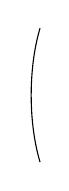
\begin{tikzpicture}
\draw (0,0) .. controls (-.15,.5) and (-.15,1.2) .. (0,1.7);
\end{tikzpicture}}
\mspage{85}

\scanpage{87}
- \mspage{IV-1008} -
\[
\psi_M:(\operatorname{gr}_\bullet(M)\otimes_A(A/\underline J))[T_1,\ldots,T_n]
 \longrightarrow\operatorname{gr}'_\bullet(M)
\]
\[
\psi_R:(\operatorname{gr}_\bullet(R)\otimes_A(A/\underline J))[T_1,\ldots,T_n]
 \longrightarrow\operatorname{gr}''_\bullet(R)
\]
\margin{\unsure{identifier aux précédents} sans
\unsure{oublier que comme d'ident des deux dernières flèches}
verticales de 19.6.1.1.}
Comme la \deleted{\unsure{gr}} filtration $(R''_k)$ est plus fine que $(R'_k)$ sur $R$, on a un
homomorphisme canonique \inserted{$\gamma:$}
$\operatorname{gr}''_\bullet(R)\longrightarrow\operatorname{gr}'_\bullet(R)$;
nous désignerons par $\psi'_R$
l'homomorphisme composé $\gamma\circ\psi_R$. Il résulte alors aussitôt des définitions
que l'on a un diagramme commutatif

\margin{orientation du diagramme \unsure{vicieuse}; à harmoniser avec 19.6.1.1.}
(19.6.2.\unsure{1})
\diagram{\begin{tikzcd}[ampersand replacement=\&,column sep=large,row sep=large,
execute at end picture={\draw (callout) to[bend left=15] (jl);
\draw (callout) to[bend left=5] (pl);}]
\&0\arrow[d]\\
(\operatorname{gr}_\bullet(R)\otimes_A(A/\underline J))[T_1,\ldots,T_n]
 \arrow[r,"\psi'_R"]
 \arrow[d,"{\operatorname{gr}(j)\otimes1}"'{name=jl,draw,ellipse}]
\&\operatorname{gr}'_\bullet(R)\arrow[d,"\operatorname{gr}'(j)"]\\
(\operatorname{gr}_\bullet(\unsure{N|M})\otimes_A(A/\underline J))[T_1,\ldots,T_n]
 \arrow[r,"\psi_N"]
 \arrow[d,"{\operatorname{gr}(p)\otimes1}"'{name=pl,draw,ellipse}]
\&\operatorname{gr}'_\bullet(N)\arrow[d,"\operatorname{gr}'(p)"]\\
(\operatorname{gr}(M)\otimes_A(A/\underline J))[T_1,\ldots,T_n]
 \arrow[r,"\psi_M"]\arrow[d]
\&\operatorname{gr}'_\bullet(M)\arrow[d]\\
0\&0\\
|[alias=callout,draw,ellipse]|\text{donner d'autres noms!}\&
\end{tikzcd}}
où les colonnes sont exactes.

\uline{Proposition\deleted{s}} (19.6.3) .- \uline{Avec les notations précédentes, supposons \inserted{que} la
suite} $f$ \inserted{soit} $\operatorname{gr}_\bullet(N)$-\uline{régulière. Considérons les conditions suivantes} :

a) $f$ \uline{est} $\operatorname{gr}_\bullet(M)$-\uline{régulière}.

b) $\psi_M$ \uline{est bijectif}.

c) $\psi'_R$ \uline{est surjectif} (autrement dit $\operatorname{gr}'_\bullet(R)$ est engendré comme
$\operatorname{gr}_{\underline J}^\bullet(A)$-module par
$\operatorname{Im}(\operatorname{gr}_\bullet(R)\longrightarrow\operatorname{gr}'_\bullet(R))$).

d) $\psi'_R$ \uline{est injectif}.

d') \uline{L'homomorphisme} $(\psi'_R)_0:
\operatorname{gr}_\bullet(R)\otimes_A(A/\underline J)\longrightarrow\operatorname{gr}'_\bullet(R)$
\uline{obtenu en restreignant} $\psi'_R$ \uline{aux polynômes de degré} $0$, \uline{est injectif}.

\deleted{\unsure{donc}} e) $\psi'_R$ \uline{est bijectif}.

f) \figure{\tikz[baseline=(a.base)]{\node[draw,ellipse](a){$\operatorname{gr}(j)\otimes1$};}}
\uline{est injectif}.

f') \uline{L'homomorphisme}
$\unsure{\operatorname{gr}_\bullet|\operatorname{gr}^\bullet_\bullet}(R)\otimes_A(A/\underline J)
 \longrightarrow\operatorname{gr}_\bullet(N)\otimes_A(A/\underline J)$
\uline{obtenu en restreignant}
\figure{\tikz[baseline=(a.base)]{\node[draw,ellipse](a){$\operatorname{gr}(j)\otimes1$};}}
\uline{aux polynômes de degré} $0$, \uline{est injectif}.

g) \uline{La filtration} $\underline J$-\uline{préadique de}
$\operatorname{gr}_\bullet(R)$ \uline{est induite par celle de}
$\operatorname{gr}_\bullet(N)$.

h) \uline{Les filtrations} $(R'_k)$ \uline{et} $(R''_k)$ \uline{sur} $R$ \uline{sont identiques}.
\mspage{86}

\scanpage{88}
Les isom de transitivité se \unsure{décomposent}
en trois isomorphismes de transitivité
particuliers :

a) deux morphismes lisses

b) Deux morphismes d'immersion,

c) commutativité des images inverses
dans le carré ($\unsure{Q|2}$). Les cas a) b)
triviaux, le cas du carré $\unsure{Q|2}$ est essentiellement
le th. de changement de base lisse.

\uline{NB.}\quad Dans tous ces isom de
transitivité, il faudrait vérifier que
quand il y a trois composés, on a les
\unsure{compatibilités|compatibilité} habituelles --- Nous l'admettrons.

\deleted{\unsure{Isom}}
2$^\circ$)\quad \uline{Formules d'adjonction}
\diagram{\begin{tikzcd}[ampersand replacement=\&,column sep=small]
X\arrow[d,no head,"f"]\&F^\bullet\\
Y\&G^\bullet
\end{tikzcd}}
\[
\boxed{\operatorname{Hom}(\mathbb{R}_!f(F^\bullet),G^\bullet)
 \simeq\operatorname{Hom}(F^\bullet,\mathbb{R}^!f(G^\bullet))}
\]
\[
[F^\bullet\in\operatorname{Ob}\mathrm D^b(X),\quad
 G^\bullet\in\operatorname{Ob}\mathrm D^+(Y)]
\]
\[
\boxed{\operatorname{Hom}(\mathbb{L}f^*(G^\bullet),F^\bullet)
 \simeq\operatorname{Hom}(G^\bullet,\mathbb{R}f_*(F^\bullet))}
\]
\[
[F^\bullet\in\operatorname{Ob}\mathrm D^+(X),\quad
 G^\bullet\in\operatorname{Ob}\mathrm D^b(Y)]
\]
\mspage{87}

\scanpage{89}
- \mspage{IV-1009} -
\uline{On a alors les implications suivantes} :
\diagram{\begin{tikzcd}[ampersand replacement=\&,column sep=small,row sep=small]
\text{a)}\arrow[r,Rightarrow]\arrow[dr,Rightarrow]
\&\text{e)}\arrow[r,Rightarrow]\arrow[dr,Rightarrow]
\&\text{b)}\arrow[r,Leftrightarrow]
\&\text{c)}\arrow[r,Leftrightarrow]
\&\text{h)}\&\\
\&\text{g)}\arrow[r,Rightarrow]
\&\text{d)}\arrow[r,Leftrightarrow]
\&\text{d')}\arrow[r,Leftrightarrow]
\&\text{f)}\arrow[r,Leftrightarrow]
\&\text{f')}
\end{tikzcd}}
\uline{En outre, lorsque tout module quotient d'un sous-module d'un}
$\operatorname{gr}_k(M)$
\uline{est séparé pour la topologie} $\underline J$-\uline{préadique}
(ce qui sera le cas lorsque
$A$ est noethérien, que les $f_i$ appartiennent au radical de $A$ et que
les $\operatorname{gr}_k(M)$ sont des $A$-modules de type fini),
\uline{alors les conditions
a) à h) sont toutes équivalentes}.

Notons que d'après (19.5.5), il résulte de l'hypothèse que $f$ est
$\operatorname{gr}_\bullet(N)$-régulière, que $\psi_N$ est \uline{bijectif};
comme $\unsure{\operatorname{gr}''(j)|\operatorname{gr}'(j)}$ est injectif,
l'équivalence de d) et f) résulte du diagramme (19.6.2.1), ainsi
que celle de d') et f'); par ailleurs f) et f') sont trivialement
équivalentes, ce qui montre l'équivalence de d),d'),f) et f').
Comme on sait déjà que $\psi_M$ est surjectif et $\psi_N$ bijectif, l'équivalence
de b) et c) découle aussi du diagramme (19.6.2.1) par un cas
particulier du lemme des cinq.

La relation $\psi'_R=\gamma\circ\psi_R$\inserted{ (19.6.2)}
et le fait que $\psi_R$ est surjectif montre\inserted{nt} que la
condition c) équivaut à dire que $\gamma$ est surjectif, ce qui équivaut
encore à la condition h); on a donc prouvé l'équivalence de b),c)
et h).

Il est trivial que e) équivaut à la \deleted{\unsure{conjonction}} conjonction de c)
et d), donc aussi de b) et d). Notons maintenant que a) implique
b) \deleted{\illegible{1}} et que b) implique a) sous l'hypothèse de séparation
(19.5.5). D'autre part, les implications a)$\Rightarrow$g)$\Rightarrow$\deleted{\unsure{f)}} f'),
et
l'implication f')$\Rightarrow$a) sous l'hypothèse de séparation, résultent de
(19.4.3). On a donc prouvé que a) entraîne e) (équivalente à la conjonction
de b) et f')), et aussi que toutes les conditions sont équivalentes
sous l'hypothèse de séparation. CQFD.

\uline{Corollaire} (19.6.4) .- \uline{Soient} $\underline K$ \uline{un idéal de} $A$,
$\underline L=\underline J+\underline K$. \uline{Supposons
que la filtration} $(N_k)$ (\uline{donc aussi} $(M_k)$)
\uline{soit la filtration} $\underline K$-\uline{\unsure{préadi-}}
\mspage{88}

\scanpage{90}
\deleted{\unsure{Pour.}} La deuxième formule est triviale,
\inserted{($f$ plat \unsure{ici, ce qui simplifie})}
\deleted{résulte}
\[
\begin{aligned}
\operatorname{Hom}(G^\bullet,\mathbb{R}f_*(F^\bullet))
 &\simeq H^0(\operatorname{Hom}^\bullet(G^\bullet,f_*(C^\bullet(F^\bullet))))\\
 &\simeq H^0(\operatorname{Hom}^\bullet(f^*G^\bullet,C^\bullet(F^\bullet)))\\
 &\simeq\operatorname{Hom}(\mathbb{L}f^*G^\bullet,F)
\end{aligned}
\]

3$^\circ$)\quad \uline{Formules de projection}
\[
\boxed{\mathbb{R}\operatorname{Hom}(\mathbb{R}_!f(F^\bullet),G^\bullet)
 \simeq \mathbb{R}f_*(\mathbb{R}\operatorname{Hom}(\mathbb{R}^!f(F^\bullet),G^\bullet))}
\]
\[
\boxed{\mathbb{R}\operatorname{Hom}(G^\bullet,\unsure{\mathbb{R}f|\mathbb{R}f_*}(F^\bullet))
 \simeq \mathbb{R}f_*(\mathbb{R}\operatorname{Hom}(\mathbb{L}f^*(G^\bullet),F^\bullet))}
\]
\[
\boxed{G^\bullet\overset{\mathbb{L}}{\otimes}\unsure{\mathbb{R}_{\deleted{\unsure{!}}}f_*|\mathbb{R}_!f}(F^\bullet)
 \simeq\unsure{\mathbb{R}_{\deleted{\unsure{!}}}f_*|\mathbb{R}_!f}
 (G^\bullet\overset{\mathbb{L}}{\otimes}F^\bullet)}
\]
\margin{\deleted{\unsure{Idem pour} $\mathbb{R}_!f(F^\bullet)$}
si $G^\bullet$ loc. libre (peut se
généraliser à $G^\bullet$ loc. \unsure{const. au $f$})}
\margin{Pour \unsure{fais}, \deleted{\unsure{on} $G^\bullet$ ``\unsure{constructible}'',
\illegible{4} \unsure{changement}, \illegible{3} $\unsure{\mathbb{R}f_*}$}}

\uline{NB}\quad Les \deleted{\unsure{for}} isom des formules 2$^\circ$, 3$^\circ$
sont associés aux hom canoniques
\[
\operatorname{Tr}_f(G^\bullet):
 \mathbb{R}_!f\,\mathbb{R}^!f(G^\bullet)\longrightarrow G^\bullet
\]
\[
\tau_f(G^\bullet):
 \deleted{\unsure{\mathbb{R}}}G^\bullet\longrightarrow(\mathbb{R}f_*(\mathbb{L}f^*(G^\bullet)))
\]
On a des énoncés de compatibilité
entre les les isom de 2$^\circ$ et 3$^\circ$, i.e. en
fin de compte les hom $\operatorname{Tr}_f$ et $\tau_f$,
\mspage{89}

\scanpage{91}
- \mspage{IV-1010} -
\uline{que, de sorte que les filtrations} $(M'_k)$ \uline{et} $(N'_k)$ \uline{sont les filtrations
L-préadiques. Considérons} $\operatorname{gr}_\bullet(R)$ (resp. $\operatorname{gr}'_\bullet(R)$)
\uline{comme un module gradué sur} $\operatorname{gr}_{\underline K}^\bullet(A)$
(resp. $\operatorname{gr}_{\underline L}^\bullet(A)$).

(i) \uline{Soit} $S$ \uline{une partie de} $\operatorname{gr}_\bullet(R)$
\uline{qui engendre} $\operatorname{gr}_\bullet(R)$ \uline{comme}
$\operatorname{gr}_{\underline K}^\bullet(A)$-\uline{module. Alors la condition c) de}
(19.6.3) \uline{équivaut à la condition suivante} :

c') \uline{L'image de} $S$ \uline{dans} \deleted{\unsure{le}}
$\operatorname{gr}'_\bullet(R)$ \uline{par} $\psi'_R$ \uline{engendre}
$\operatorname{gr}'_\bullet(R)$ \uline{comme} $\operatorname{gr}_{\underline L}^\bullet(A)$-\uline{module}.

(ii) \uline{Supposons vérifiée la condition e) de} (19.6.3), \uline{et de plus que
les quotients des} $\operatorname{gr}_k(R)$ \uline{soient séparés pour la topologie}
$\underline J$-\uline{préadique} (ce qui sera le cas lorsque $A$ est noethérien,
les $f_i$ dans le radical de $A$ et les $\operatorname{gr}_k(N)$ des $A$-modules de type fini).
\uline{Alors, pour
qu'une partie} $S$ \uline{de} $\operatorname{gr}_\bullet(R)$
\uline{formée d'éléments homogènes engendre} $\operatorname{gr}_\bullet(R)$
\uline{comme} $\operatorname{gr}_{\underline K}^\bullet(A)$-\uline{module,
il faut et il suffit que son image par} $\psi'_R$ \uline{engendre}
$\operatorname{gr}'_\bullet(R)$ \uline{comme}
\deleted{$\unsure{\operatorname{gr}_{\underline K}^\bullet(A)}$}
$\operatorname{gr}_{\underline L}^\bullet(A)$-\uline{module}.

(i) Considérons l'homomorphisme \deleted{\unsure{canonique}} de degré 0
\[
\psi_A:(\operatorname{gr}_{\underline K}^\bullet(A)\otimes_A(A/\underline J))[T_1,\ldots,T_n]
 \longrightarrow\operatorname{gr}'_\bullet(A)=\operatorname{gr}_{\underline L}^\bullet(A)
\]
(\uline{0},15.1.5.2). Le fait que cet homomorphisme soit \uline{surjectif} entraîne
que la sous-$\operatorname{gr}_{\underline L}^\bullet(A)$-algèbre de
$\operatorname{gr}'_\bullet(R)$ engendrée par $S'=\psi'_R(S)$ n'est
autre que \deleted{$\unsure{\operatorname{gr}_\bullet(R)}$}
$\operatorname{Im}(\psi'_R)$, d'où l'équivalence de c) et c').

(ii) Puisque e) est vérifiée, il en est de même de c), et en vertu
de (i), il reste à prouver la suffisance de la condition de l'énoncé.
Or, comme $\psi'_R$ est bijectif, dire que $S'$ engendre
$\operatorname{gr}'_\bullet(R)$ considéré comme
$\operatorname{gr}_{\underline L}^\bullet(A)$-module équivaut à dire que $S$ engendre
$(\operatorname{gr}_\bullet(R)\otimes_A(A/\underline J))[T_1,\ldots,T_n]$
comme \deleted{$\unsure{\operatorname{gr}_{\underline K}^\bullet(A)}$}
$\operatorname{gr}_{\underline L}^\bullet(A)$-module, et en vertu
de la surjectivité de $\psi_A$, on peut dans cet énoncé remplacer
l'anneau $\operatorname{gr}_{\underline L}^\bullet(A)$ par
$(\operatorname{gr}_{\underline K}^\bullet(A)\otimes_A(A/\underline J))[T_1,\ldots,T_n]$.
Il revient évidemment
au même de dire que $S$ engendre
$\unsure{\{|f}\operatorname{gr}_\bullet(R)\otimes_A(A/\underline J)$ en tant que module sur
l'anneau $\operatorname{gr}_{\underline K}^\bullet(A)\otimes_A(A/\underline J)$,
ou aussi en tant que $\operatorname{gr}_{\underline K}^\bullet(A)$-module..
\deleted{\unsure{nous}}\inserted{Or,}
\mspage{90}

\scanpage{92}
et les isom de transitivité de $1^\circ$ \unsure{\ldots}

$-$

$4^\circ)$ Formules de changt de base (auraient intérêt \unsure{à être|: être} bloquées après $1^\circ$)

\diagram{\begin{tikzcd}[ampersand replacement=\&]
X \& X' \arrow[l,"g'"']\\
Y \& Y' \arrow[l,"g"] \arrow[u,phantom]
\arrow[from=1-1,to=2-1,"f"'] \arrow[from=1-2,to=2-2,"f'"]
\end{tikzcd}}

\[
\boxed{\boxed{\mathbb{L}g^*\mathbb{R}_!f_*\xrightarrow{\sim}\mathbb{R}_!f'_*\mathbb{L}g'^*}}
\]
\margin{ch. de base pour morphismes \uline{propres}}
\margin{\figure{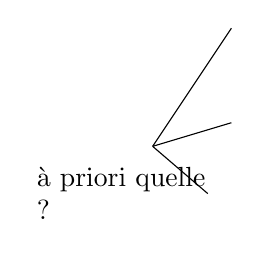
\begin{tikzpicture}
\draw (0,0)--(1,1.5);
\draw (0,0)--(1,.3);
\draw (0,0)--(.7,-.6);
\node[align=left] at (-.4,-.6) {\unsure{à priori quelle}\\\unsure{?}};
\end{tikzpicture}}}
\[
\left\{
\begin{aligned}
\mathbb{L} g^{\deleted{\unsure{*}}*}\mathbb{R}f_*&\xrightarrow{\sim}\mathbb{R}f'_*\mathbb{L}g'^*
&&\text{si $f$ propre \boxed{\text{ou $g$ lisse}}}\\
\uuline{\mathbb{R}^{\inserted{!}}f^{\deleted{\unsure{*}}\inserted{'}}\mathbb{L}g^*}
&\uuline{\xleftarrow{\sim}\deleted{\unsure{\mathbb{R}^*}}\inserted{\mathbb{L}}g'^*\mathbb{R}^{\inserted{!}}f^{\deleted{\unsure{*}}}}
&&\text{si $f$ ou \boxed{\text{$g$ lisse}}}
\end{aligned}
\right.
\]
\figure{\begin{tikzpicture}
\node (a) at (0,0) {$\boxed{\mathbb{R}^!g\mathbb{R}_!^{\deleted{\unsure{*}}}f\xrightarrow{\sim}\mathbb{R}_!^{\deleted{\unsure{*}}}f'\mathbb{R}^!g'}$};
\draw[decorate,decoration={snake,amplitude=1pt,segment length=12pt}] (-3.0,-.4) rectangle (3.0,.4);
\node at (5.0,0) {si $f$ propre ou $g$ lisse};
\node[draw,double] (b) at (0,-1.2) {$\mathbb{R}^!g\mathbb{R}f_*\simeq \mathbb{R}f'_*\mathbb{R}^!g'$};
\draw[<->] (-3.6,.4) -- (-3.6,-1.5);
\node[rotate=22] at (-4.0,.5) {$g$ lissifiable};
\node[align=left] (c) at (7,-1.1) {$\Leftrightarrow$ (\unsure{se décompose en cas lisse}\\
$={}$ changt de base lisse, et cas d'une\\
immersion, trivial)};
\node[align=left] (d) at (6.7,1.2) {changt de\\base lisse};
\draw[<->] (6.7,1.7) -- (6.7,2.3);
\draw[->] (d.east) to[bend left=35] (c.north east);
\node (e) at (1,-2.5) {est une conséquence du précédent};
\draw[->] (-3.2,.5) to[bend right=30] (e.west);
\end{tikzpicture}}

$5^\circ)$ \uline{Formules d'induction}
\[
\boxed{\mathbb{R}^!f(\mathbb{R}\operatorname{Hom}(F^\bullet,G^\bullet))
\simeq \mathbb{R}\operatorname{Hom}(\mathbb{L}f^*(F^\bullet),\mathbb{R}^!f(G^\bullet))}
\]
\diagram{\begin{tikzcd}[ampersand replacement=\&]
X\arrow[d,"f"]\\
Y\quad F,G
\end{tikzcd}}
\[
\boxed{\mathbb{L}f^*(F^\bullet\mathbin{\overset{\mathbb{L}}{\otimes}}G^\bullet)
\simeq \mathbb{L}f^*(F^\bullet)\mathbin{\overset{\mathbb{L}}{\otimes}}\mathbb{L}f^*(G^\bullet)}
\]
\margin{formule pour topos annelés quelconques \unsure{\ldots}}
\mspage{91}

\scanpage{93}
- \mspage{IV-1012} -
L'implication a)$\Rightarrow$c) est immédiate \deleted{\illegible{1}} (\uline{0},15.1.13). Si c) est vérifiée, il résulte de (19.5.5) que $\psi_M$ est bijectif ; en outre,
\deleted{\unsure{$\operatorname{gr}_{\underline K}^\bullet(M)$} \illegible{6}}
$(\operatorname{gr}_{\underline K}^\bullet(M)\otimes_A(A/\underline J)=
=(\operatorname{gr}_{\underline K}^\bullet(M)\otimes_{A/\underline K}(A/\underline L)\unsure{)|/}$ est un $(A/\underline L)$-module plat, donc il en est de même de
$(\operatorname{gr}_{\underline K}^\bullet(M)\otimes_A(A/\underline J))[T_1,\ldots,T_n]$, et par suite de $\operatorname{gr}_{\underline L}^\bullet(M)$ puisque $\psi_M$ est un $(A/\underline L)$-isomorphisme ; donc c) entraîne b). Le fait que a) implique b) montre aussitôt que a) implique aussi d).
\margin{/(Bourbaki, \uline{Alg.}, chap. II, $3^\mathrm{e}$ éd., § 3, n° 7, cor. 2 de la prop. 6)}

Lorsque tout quotient d'un $\operatorname{gr}_{\underline K}^p(M)$ est idéalement séparé pour $\underline J$, il résulte de (19.5.5) que la condition b) entraîne que $f$ est $(\operatorname{gr}_{\underline K}^\bullet(M))$-régulière ; en outre, comme
$(\operatorname{gr}_{\underline K}^\bullet(M)\otimes_{A/\underline K}(A/\underline L))[T_1,\ldots,T_n]$, isomorphe à $\operatorname{gr}_{\underline L}^\bullet(M)$, est alors un $(A/\underline L)$-module plat, \deleted{\unsure{et}} il en est \deleted{\illegible{1}} de même de
$\operatorname{gr}_{\underline K}^\bullet(M)\otimes_{A/\underline K}(A/\underline L)$, qui en est un facteur direct ; cela prouve donc que b) entraîne alors c). D'autre part, c) entraîne alors a) en vertu de (\uline{0},15.1.21) (où on peut remplacer l'hypothèse noethérienne par l'hypothèse que $M$ est idéalement séparé pour $\underline J$, en vertu de $(\underline{0_{\mathrm{III}}},10.2.1)$).

Il reste donc à prouver que lorsque $A$ est noethérien, $M$ de type fini et que les \deleted{\illegible{1}} $f_i$ appartiennent au radical de $A$, d) entraîne a). Il existe par hypothèse un $A$-module \uline{libre de type fini} \inserted{$N$} et une suite exacte
$0\longrightarrow R\longrightarrow N\longrightarrow\unsure{M}\longrightarrow0$.
Il suffit de prouver que d) entraîne b), puisque tout quotient d'un sous-module d'un $\operatorname{gr}_{\underline K}^p(M)$ est alors idéalement séparé pour $\underline J$, en vertu du fait que $\operatorname{gr}_{\underline K}^p(M)$ est un $A$-module de type fini \deleted{\illegible{1}}, que $\underline J$ est contenu dans le radical de $A$, \deleted{\illegible{1}} et que $A$ est noethérien (Bourbaki, \uuline{Alg. comm.}, chap. III, § 5, n° 1) ; en d'autres termes, il s'agit de voir que $\psi_M$ est \uline{bijectif}.
\deleted{\illegible{5}}
\mspage{92}

\scanpage{94}
Établissons la première formule d'induction.

On distingue les cas $f$ \uline{lisse}, et $f$ une immersion fermée.

a) \uline{Cas} $f$ \uline{lisse}. La formule équivaut à :
\[
\mathbb{L}f^*(\mathbb{R}\operatorname{Hom}(F^\bullet,G^\bullet))
\simeq \mathbb{R}\operatorname{Hom}(\mathbb{L}f^*_{\unsure{s}}F^\bullet,\mathbb{L}f^*G^\bullet)
\]
i.e. au fait que \uline{si $f$ est lisse}, \deleted{\unsure{$\mathbb{L}$}}$f^*$ \uline{commute aux} $\operatorname{Ext}^i$ \uline{locaux},
\inserted{(\unsure{si le premier est} \deleted{\unsure{borné}})}
à degrés bornés [sup.] \deleted{et à \unsure{degré|de} type \uline{constructible}}. On a en tous cas une flèche évidente $\longrightarrow$, à prouver que c'est un isomorphisme.

\deleted{\unsure{C'est local, on peut supposer} $Y,X$ affines, par \unsure{passage à la limite on peut supposer que} $Y$ \unsure{est noethérien}. On peut supposer que}

On peut supposer $Y,X$ affines, $F^\bullet$ réduit au degré $0$, \inserted{$G^\bullet$ itou et injectif.}
\deleted{Alors $F$ admet une filtration \inserted{finie} par des
\inserted{$F'$ loc. constant sur $Y'$},
\deleted{\unsure{$\mathbb{R}$}}$i_!(\unsure{F'|G'})$, où $i:Y'\unsure{-|\longrightarrow}Y$ immersion,
\inserted{\unsure{donc pour}}
\unsure{tout ceci on peut supposer que|toute cette on peut supposer que}
$F=\deleted{\unsure{\mathbb{R}}}i_!\unsure{G'|F'}$,
$F'$ loc. constant.}
\margin{\deleted{\unsure{si fini}}}
\deleted{On \unsure{a une présentation} de $F$ par une
\inserted{\unsure{somme directe de}}
$(\mathbb{R}i_!(\Lambda_{Y'}))$, $Y'\unsure{-|\longrightarrow}Y$
\deleted{\unsure{étale}} étale \unsure{affine},
\unsure{de là que cela revient au cas où}.}
\mspage{93}

\scanpage{95}
\mspage{111}
In the case where $W=V$, $f_1:V\longrightarrow V$ is the identity and $f_o$ is the constant map, (7) reduces to the formula required in Appendix I.

The above considerations may be applied to obtain a homotopy formula for $d_\tau$, $\tau\in Y$ (see §5.2) analogous to (7) provided that $U,V,W$ and the map $f$ satisfy the additional requirement imposed by the structure and provided in addition that $U$ is pseudo-Kählerian (for example, if $U,V,W$ and the map $f$ are complex-analytic, $U$ Kählerian). The construction is based on the operator $M_{\tau,o}$, $\tau\in Y$. If the operator $M_{\tau,o}$ exists for $\tau=\sqrt{-1}$, the above argument also applies but with the difference that the term $(F_n)_U\varphi/c$ no longer vanishes. In this case $(F_n)_U=F_U$ signifies projection onto functions which are holomorphic in their dependence on the point of $U$ and we obtain the formula
\[
(\bar\partial\lambda+\lambda\bar\partial)\varphi
=f_1^*\varphi-f_o^*\varphi-((F_Uf^*)_1-(F_uf^*)_o)\varphi.
\]

The necessity of the additional terms involving $F_U$ is shown by examples (see [14]).
\mspage{94}

\scanpage{96}
\[
f^*(\unsure{F'|F})=j_!\bigl(\underbrace{f'^*(F')}_{F'_{X'}}\bigr)
\]
\diagram{\begin{tikzcd}[ampersand replacement=\&]
X'\arrow[r,hook,-,"j"]\arrow[d,"f'"']\&X\arrow[d,"f"]\\
Y'\arrow[r,hook,"i"']\&Y\\
F'
\end{tikzcd}}
\[
\overbrace{\mathbb{R}\operatorname{Hom}(\mathbb{R}i_!(F'),G^\bullet)}^{\Vert}
\overset{\text{\uline{dualité pour $i$}}}{\simeq}
\mathbb{R}i_*\bigl(\mathbb{R}\operatorname{Hom}(F',\mathbb{R}i^!(G^\bullet))\bigr)
\]
\[
\begin{aligned}
\mathbb{L}f^*(\hspace{2.5cm})&\simeq \mathbb{L}f^*\mathbb{R}i_*(\hspace{3cm})\\
&\underset{\text{ch. de base lisse}}{\simeq}
\mathbb{R}j_*\underbrace{\mathbb{L}f'^*\bigl(\mathbb{R}\operatorname{Hom}(F',\mathbb{R}i^!(G^\bullet))\bigr)}_{
\begin{gathered}
\Vert\quad\text{supposons un instant}\\
\text{(i.e. th. vrai pour $f':X'\unsure{-|\longrightarrow}Y'$ et $F',\mathbb{R}i^!G^\bullet$)}
\end{gathered}}
\end{aligned}
\]
\[
\mathbb{R}\operatorname{Hom}\bigl(f'^*(F'),
\underbrace{f'^*(\mathbb{R}i^!(G^\bullet))}_{
\begin{gathered}
\Vert\quad\text{--- th. de chang. de base lisse}\\
\mathbb{R}j^!(f'^*(G^\bullet))
\end{gathered}}\bigr)
\]
\[
\begin{aligned}
&\simeq \mathbb{R}j_*\bigl(\mathbb{R}\operatorname{Hom}(F'_{\unsure{X'|X}},\mathbb{R}j^!G_X^\bullet)\bigr)\\
&\underset{\text{dualité pour $j$}}{\simeq}
\mathbb{R}\operatorname{Hom}\bigl(\underbrace{j_!F'_{\unsure{X'|X}})}_{
f^{\inserted{*}}_{\deleted{\unsure{*}}}(F_{\deleted{\unsure{X}}})},G_X^\bullet\bigr)\\
&\simeq \mathbb{R}\operatorname{Hom}\bigl(\mathbb{L}f^*(F_X),f^*(G)\bigr)
\end{aligned}
\]
\deleted{\unsure{$f^*$}}

On est ramené donc au cas où $F$ est loc. constant. On peut donc (le thm \unsure{étant} local)
\mspage{95}

\scanpage{97}
\mspage{73}
Again note that $\mathbb S_x\mathbb H_xJ$ is represented by the matrix whose elements are the symbols of theelements of the matrix corresponding to $\mathbb H_xJ$. Thus, if $\xi(x)$ is represented by $(\xi^{ij})$ and $F_x$ by $(F^{ij})$, then we obtain

\uline{Theorem 4.6.8.} If $F^{ij}=\displaystyle\sum_{n=1}^{\infty}Y_n^{ij}$, where $Y_n^{ij}$ is a spherical harmonic of degree $n$, then
\[
(\mathbb S_x\mathbb H_xJ)(u)=\xi^{ij}+\sum_{n=1}^{\infty}\gamma_nY_n^{ij}(u),
\quad u\in S_x
\]
where
\[
\gamma_n=i^n\pi^{\frac m2}\frac{\Gamma(\frac n2)}{\Gamma(\frac{m+n}{2})}.
\]

If $J\in\mathcal G^p$, we again say that $J\rho=\alpha$ is regularizable if there exists $K\in\mathcal G^p$ such that $KJ\rho=K\alpha$ is a Fredholm equation with the same solutions as $J\rho=\alpha$. Now by applying the results of systems of singular equations, see [20f] pp. 106-109, we get

\uline{Theorem 4.6.9.} If $J\in\mathcal G^p$ then the equation $J\rho=\alpha$ is regularizable if and only if
$\det[\mathbb S_x\mathbb H_xJ(u)]\ne0$ for all $u\in S_x$ and all $x\in M$.

Now let $\mathcal S_M^p$ be the algebra of bundle maps of $S(M)\longrightarrow A^p\otimes A^p$. We define a map
$\mathbb S_M:\mathcal G^p\longrightarrow\mathcal S_M^p$ by
\mspage{96}
